\section{Object reconstruction}

We review the properties of the particles most pertinent to the analyses presented in this work (taus, muons, electrons, jets, and b-jets), their signatures in the CMS detector, and dedicated reconstruction techniques used at CMS.

\subsection{Taus}
The tau ($\tau$) is the heaviest known lepton. With a rest mass of 1776.86 MeV, it can decay to not only electrons and muons, but also hadrons. The mean lifetime of the $\tau$ is $\tau = 290 \times 10^{-15}$ seconds, corresponding to $c\tau = 87.03$ $\mu$m, which is short enough that taus decay in the CMS detector before reaching the detector elements. 

In two thirds of the cases, $\tau$ leptons decay hadronically, typically into one or three charged mesons (predominantly $\pi^+$, $\pi^-$), often accompanied by neutral pions (that decay $\pi^0 \rightarrow \gamma\gamma$), and a $\nu_{\tau}$. These hadronic decays are denoted $\tau_{h}$. In the remainder of the decays, the tau decays to the lighter leptons (electron or muon), termed leptonic decays. In all cases, at least one neutrino is produced, resulting in missing transverse energy in the CMS detector. The tau's largest decay branching ratios (proportional to probability of decay) are listed below \citep{workman_review_2022}: 
\begin{itemize}
    \item 17.8\% decay to $e^- \bar{\nu}_e \nu_{\tau}$
    \item 17.4\% decay to $\mu^- \bar{\nu}_\mu \nu_{\tau}$
    \item 25.5\% decay to $\pi^- \pi^0 \nu_{\tau}$ ($\rho^-$ resonance at 770 MeV)
    \item 10.8\% decay to $\pi^- \nu_{\tau}$ % (excluding $K^0, \omega$)
    \item 9.3\% decay to $\pi^- \pi^0 \pi^0 \nu_{\tau}$  ($a_1^-$ resonance at 1200 MeV)
    \item 9.0\% decay to $\pi^- \pi^- \pi^+ \nu_{\tau}$ ($a_1^-$ resonance at 1200 MeV)
\end{itemize}

The neutrinos escape undetected from the CMS detector and are not considered in the reconstruction. Charged hadrons leave tracks in the tracking detector before being absorbed in the hadronic calorimeter; in CMS tau reconstruction terminology, they are often called ``prongs'', i.e. the dominant $\tau_{h}$ decay modes are termed ``1 prong" ($\pi^\pm$), ``1 prong + $\pi^0$(s)", and ``3-prong''. Neutral pions decay to two photons which lose their energy in the electromagnetic calorimeter. Taus that decay to electrons and muons, are typically triggered on and reconstructed as electrons and muons respectively. 

\subsubsection{Hadron plus strips (HPS) reconstruction of $\tau_{h}$}
At CMS, hadronically decaying tau leptons are reconstructed with the hadron plus strips (HPS) algorithm \citep{CMS-TAU-14-001} \cite{2012-JINST-7-P01001}. The HPS algorithm capitalizes on photon conversions in the CMS tracker material, which originate from the neutral pion ($\pi^0$) decaying to two photons. The bending of electron/positron tracks due to the CMS solenoid magnetic field leads to a spread of the neutral pions' calorimeter signatures in the $\phi$ direction. This motivates the reconstruction of photons in ``strips": objects that are built out of PF photons and electrons. The strip reconstruction starts with centering a strip on the most energetic electromagnetic particle in a PF jet. Among other electromagnetic particles located in a window of size $\Delta \eta = 0.05$ and $\Delta \phi = 0.20$ around the strip center, the most energetic one is associated with the strip and its momentum is added to the strip momentum. This is repeated iteratively until no further particles can be associated. Lastly, strips satisfying a requirement of $p_{T}^{\text{strip}} > 1$ GeV are combined with charged hadrons to reconstruct individual $\tau_{h}$ decay modes, where $h$ stands for both $\pi$ and $K$:
\begin{itemize}
    \item \textit{Single hadron}: $h^- \nu_{\tau}$ and $h^- \pi^0 \nu_{\tau}$ decay modes, in which the neutral pions have too little energy to be reconstructed as strips.
    \item \textit{One hadron + one strip}: $h^- \pi^0 \nu_{\tau}$ decay modes, where the photons from the $\pi^0$ decay are close together in the calorimeter.
    \item \textit{One hadron + two strips}: $h^- \pi^0 \nu_{\tau}$ decay modes, where the photons from the $\pi^0$ decay are well separated. 
    \item \textit{Three hadrons}: $h^- h^+ h^- \nu_{\tau}$ decay modes. The three charged hadrons are required to originate from the same secondary vertex.
\end{itemize}
The $h^- \pi^0 \pi^0 \nu_{\tau}$ and $h^- h^+ h^- \pi^0 \nu_{\tau}$ decay modes do not have their own treatment are reconstructed with the above topologies. 

In the HPS algorithm, the direction of the reconstructed tau momentum $\vec{p}^{\tau_{h}}$ is required to fall within a distance of $\Delta R = 0.1$ from the original PF jet. All charged hadrons and strips are required to be contained within a cone of size $\Delta R = (2.8 \,\text{GeV})/p_{T}^{\tau_{h}}$, from the $\tau_{h}$ as reconstructed by the HPS. 

All charged hadrons are assumed to be pions, and they are required to be consistent with the masses of the intermediate meson resonances (if applicable), with the following allowed windows for candidates: 50-200 MeV for $\pi^0$, 0.3-1.3 GeV for $\rho$, and 0.8-1.5 GeV for $a_1$. If the $\tau_{h}$ decay is compatible with more than one hypothesis, the one giving the highest $p_{T}^{\tau_{h}}$ is chosen. Lastly, an isolation requirement is applied: aside from the $\tau_{h}$ decay products, no charged hadrons or photons can be present within an isolation cone of size $\Delta R = 0.5$ around the direction of the $\tau_{h}$. The outputs of the HPS algorithm are the reconstructed decay mode and the visible four-momentum (i.e. the four-momenta of all decay products excluding the neutrinos).

\subsubsection{DeepTau for identifying $\tau_{h}$}
The identification of $\tau_{h}$ candidates in CMS has historically been divided into separate discriminators against jets, electrons, and muons. Discriminators versus jets and electrons use information from derived quantities, such as the $p_{T}$ sum of particles near the $\tau_{h}$ axis. Building on the previous multivariate analysis (MVA) classifier \cite{CMS-TAU-16-003} based on a boosted decision tree (BDT), DeepTau is a more recent classifier based on a deep neural network (DNN) that simultaneously discriminates against jets, electrons, and muons. The DNN uses a combination of high-level inputs, similar to previous algorithms, and also uses convolutional layers in $\eta$-$\phi$ space to process information from all reconstructed particles near the $\tau_{h}$ axis. Convolutional layers are based on the principle that an image can be processed independently of its position. 

The final DeepTau discriminators against jets, muons, and electrons are given by 
\begin{equation}
    D_\alpha(y) = \frac{y_{\tau}}{y_{\tau} + y_{\alpha}}
\end{equation}
where $y_\tau$ ($y_\alpha$) are estimates of the probabilities for the $\tau_{h}$ candidate to come from a genuine $\tau_{h}$ (jet, $\mu$, $e$). Working points for each discriminator with different $\tau_{h}$ identification efficiencies are defined for $D_{e}$, $D_{\mu}$, and $D_{\text{jet}}$, for usage in physics analyses and derivation of data-to-simulation corrections \cite{2022-PRD-DeepTau}. 

\subsection{Muons}
\label{section:ch-5-muon-reconstruction}
Muons are the next lightest lepton after taus, with a mass of $105.66$ MeV and a mean lifetime of $\tau = 2.20 \times 10^{-6}$ seconds, or $c\tau = 658.64$ m. At CMS, muons are identified with requirements on the quality of the track reconstruction and on the number of measurements in the tracker and the muon systems \citep{CMS-MUO-10-004}. In the standard CMS reconstruction, tracks are first reconstructed independently in the inner tracker (tracker track) and in the muon system (standalone-muon track). Next, these tracks are processed in two different methods.

The first is Global Muon reconstruction (outside-in) \citep{CMS-MUO-10-004}, which fits combined hits from the tracker track and standalone-muon track, using the Kalman-filter technique. At large transverse momenta, $p_{T} \gtrsim 200$ GeV, the global-muon fit can improve the momentum resolution compared to the tracker-only fit. 

The second is Tracker Muon reconstruction (inside-out) \citep{CMS-MUO-10-004}, which starts with tracker tracks with $p_{T} > 0.5$ GeV and total momentum $p_{T} > 2.5$ GeV. These tracks are extrapolated outwards to the muon system and matched to detector segments there, taking into account the magnetic field, expected energy losses, and multiple Coulomb scattering in the detector material. Tracker Muon reconstruction is more efficient than the Global Muon reconstruction at low momenta, $p \lesssim 5$ GeV, because it only requires a single muon segment in the muon system, where as Global Muon reconstruction typically requires segments in at least two muon stations.

To further suppress fake muons from decay in flight, isolation cuts are used. A relative isolation variable is defined to quantify the energy flow of particles near the muon trajectory.
A relative isolation is defined similarly for muons and electrons:
\begin{equation}
    I^\ell \equiv \frac{\sum_{\text{charged}} p_{T} + \text{max}\left( 0, \sum_{\text{neutral}} p_{T} - \frac{1}{2}  \sum_{\text{charged, PU}} p_{T}  \right)}{p_{T}^\ell}
    \label{eqn:definition-relative-isolation}
\end{equation}
where $\sum_{\text{charged}} p_{T}$ is the scalar sum of the $p_{T}$ of the charged particles originating from the primary vertex and located in a cone of size $\Delta R = \sqrt{(\Delta \eta)^2 + (\Delta \phi)^2} = 0.4 (0.3)$ centered on the direction of the muon (electron). The sum $\sum_{\text{neutral}} p_{T}$ is the equivalent for neutral particles. The sum $\sum_{\text{charged, PU}} p_{T}$ is the scalar sum of the $p_{T}$ of the charged hadrons in the cone originating from pileup vertices. The factor $1/2$ comes from simulation estimations, which find that the ratio of neutral to charged hadron production in the hadronization process of inelastic $pp$ collisions is $1/2$. Thus the subtracted term is intended to subtract contribution from pileup, from the neutral particle contribution to the isolation sum. Finally, this is divided by the lepton transverse momentum, $p_{T}^\ell$. 


\subsection{Electrons}
Electrons are the lighest lepton with a mass of $0.511$ MeV. At CMS, electrons are reconstructed by associating a track reconstructed in the silicon tracking detector with a cluster of energy in the ECAL. Performance is maximized via a combination of a stand-alone approach and the complementary global particle-flow approach \citep{JINST-2015-10-P06005}. 

In the stand-alone approach, the electron energy, which is typically spread over several crystals of the ECAL, is clustered with the ``hybrid'' algorithm in the barrel and the ``multi-$5\times 5$'' in the endcaps \citep{JINST-2015-10-P06005}. The hybrid algorithm collects energy in a small window in $\eta$ and an extended window in $\phi$. It identifies a seed crystal, and adds arrays of $5 \times 1$ crystals in $\eta \times \phi$ in a range of $N = 17$ crystals in both directions of $\phi$, if their energies exceed a minimum threshold, thus forming a supercluster (SC).  In the endcap, crystals are not arranged in an $\eta \times \phi$ geometry; instead clusters are build around seed crystals in clusters of $5\times 5$ crystals that can partly overlap. Nearby clusters are grouped into a supercluster, and energy is recovered from associated deposits in the preshower. 

In the PF reconstruction \citep{JINST-2015-10-P06005}, PF clusters are reconstructed by aggregating around a seed all contiguous crystals with energies two standard deviations above the electronic noise observed at the beginning of a data-taking run. The energy of a given crystal can be shared among two or more clusters.

The electron track reconstruction is performed in two ways \citep{JINST-2015-10-P06005}: the ECAL-based seeding, which begins with the SC energy and positioning, and the tracker-based seeding (part of the PF reconstruction algorithm), which uses tracks reconstructed from the general algorithm for charged particles, extrapolated towards the ECAL and matched to an SC. Kalman filter (KF) tracks with a small number of hits or that are not well-fitted, are re-fitted with a dedicated Gaussian sum Filter (GSF).

A global identification variable \citep{JINST-2015-10-P06005} is defined using a multivariate analysis (MVA) technique that combines information on track observables (kinematics, quality of the KF track and GSF track), the electron PF cluster observables (shape and pattern), and the association between the two (geometric and kinematic observables). For electrons seeded only through the tracker-based approach, a weak selection is applied on this MVA variable. For electrons seeded through both approaches, a logical OR is taken. 

Electron isolation, i.e. the presence of energy deposits near the electron trajectory, is a separate key handle in rejecting significant background. Compared to isolated electrons, electrons from misidentified jets or genuine electrons within a jet resulting from semileptonic decays of $b$ or $c$ quarks tend to have significant energy deposits near the primary trajectory \citep{JINST-2015-10-P06005}. Offline analyses benefit from the PF technique for defining isolation, which sums the PF candidates reconstructed located within a specified isolation cone around the electron candidate, as in Eqn. \ref{eqn:definition-relative-isolation}.

\subsection{Jets}
The vast majority of processes of interest at the LHC contains quarks or gluons in the final state, but these particles cannot be observed directly. In a process called hadronization, they fragment into spatially-grouped collections of particles called jets, which can be detected in the tracking and calorimeter systems. Hadronization and the subsequent decays of unstable hadrons can produce hundreds of nearby particles in the CMS detector. Jets are reconstructed by the PF algorithm (PF jets), or from the sum of the ECAL and HCAL energies deposited in the calorimeter towers (Calo jets). In PF jets, typically used in offline analyses, jets are built using the anti-$k_T$ (AK) clustering algorithm \cite{CMS-BTV-12-001}. The anti-$k_T$ algorithm iterates over particle pairs and finds the two that are closest in a distance measure $d$, and determines whether to combine them:
\begin{equation}
    d_{ij} = \text{min} \left(p_{T, i}^{-2}, \, p_{T, j}^{-2} \right) \frac{\Delta_{ij}^2}{R^2}, \, \,
    \text{combine when $d_{ij} < p_{T,i}^{-2}$; stop when $d_{ij} > p_{T, i}^{-2}$}
    \label{eqn:anti-kT}
\end{equation}
where $\Delta_{ij}^2 = (\eta_i - \eta_j)^2 + (\phi_i - \phi_j)^2$ and $p_{T, i}$, $\eta_i$, $\phi_i$ are the transverse momentum, rapidity, and azimuthal angle of particle $i$. The power $-2$ means that higher-momentum particles are clustered first, leading to jets that tend to be centered on the hardest (highest $p_T$) particle.

There are several methods to remove contributions of pileup collisions from jet clustering \cite{CMS-PAS-JME-14-001}:
\begin{itemize}
    \item Charged hadron subtraction (CHS), which removes all charged hadron candidates associated with a track that is not associated with the primary vertex.
    \item PileUp Per Particle Identification (PUPPI), which weighs input particles based on their likelihood of arising from pileup. QCD particles tend to have a collinear structure, compared to soft diffuse radiation coming from pileup. The local shape for charged pileup, used as a proxy for all pileup particles, is used on an event-by-event basis to calculate a weight for each particle. PUPPI is deployed in Run-2 and is more performant than CHS in high pileup scenarios.
\end{itemize}

\subsection{B jets}
Jets that arise from bottom-quark hadronization (b jets) have overwhelming background from processes involving jets from gluons (g) and light-flavour quarks (u, d, s), and from c-quark fragmentation. The ability to identify b jets, or b-tagging, exploits the b hadrons' relatively large masses, long lifetimes, and daughter particles with hard momentum spectra \cite{CMS-BTV-12-001}. 

The impact parameter (IP) of a track is the 3-dimensional distance between the track and the primary vertex (PV) at the point of closest approach. The IP is positive if the track originates from the decay of particles travelling along the jet axis. The resolution of the IP depends on the $p_{T}$ and $\eta$ of the track, motivating the use of the impact parameter significance $S_{\text{IP}}$ (ratio of the IP to its estimated uncertainty) as an observable \cite{CMS-BTV-12-001}.

Because of the large but finite lifetimes of the b hadrons, b hadrons tend to travel a short distance before decaying at a secondary vertex (SV), which can be measured and reconstructed separately from the primary vertex due to the excellent position resolution of the pixel detector \cite{CMS-BTV-12-001}. Previous b-tagging algorithms (e.g. CSV, cMVAv2, and DeepCSV) have capitalized on variables such as the presence of a SV, the flight distance and direction (computed from the vector between the PV and the SV), and kinematics of the system of associated secondary tracks (e.g. track multiplicity, mass, and energy). 

The DeepJet (formerly known as DeepFlavour) algorithm \cite{CMS-DP-2017-013} is a deep-neural-network multi-classification algorithm, which uses 16 properties of up to 25 charged and 6 properties of 25 neutral particle-flow jet constituents, as well as 17 properties from up to 4 secondary vertices associate with the jet. Compared to the previous classifying algorithm DeepCSV, DeepJet has been demonstrated to have higher efficiency with lower misidentification probability in Phase-1 data \cite{CMS-DP-2018-058}. 



\section{Reconstruction of the $\tau\tau$ mass}

The final signal extraction is done to the total $\tau\tau$ mass, which is estimated from the visible $\tau\tau$ mass using the FastMTT algorithm \cite{2014_SVFit_Bianchini}. FastMTT is based on the SVFit algorithm, originally developed for the Standard Model $H \rightarrow \tau\tau$ analysis \cite{CMS-HIG-13-004}. Both the SVFit algorithms, and the FastMTT algorithm, are described below, to give a complete picture of how tau decays are parameterized.

To specify a hadronic $\tau$ decay, six parameters are needed \cite{CMS-HIG-13-004}: the polar and azimuthal angles of the visible decay product system in the $\tau$ rest frame, the three boost parameters from the $\tau$ rest frame to the laboratory frame, and the invariant mass $m_{\text{vis}}$ of the visible decay products. For a leptonic $\tau$ decay, two neutrinos are produced, and a seventh parameter, the invariant mass of the two-neutrino system, is necessary. The unknown parameters are constrained by four observables that are the components of the four-momentum of the system formed by the visible decay products of the $\tau$ lepton, measured in the laboratory frame. The remaining unconstrained parameters for hadronic and leptonic $\tau$ decays are thus:

\begin{itemize}
    \item The fraction of the $\tau$ energy in the laboratory frame carried by the visible decay products,
    \item $\phi$, the azimuthal angle of the $\tau$ direction in the laboratory frame,
    \item $m_\nu\nu$, the invariant mass of the two-neutrino system in leptonic $\tau$ decays (for hadronic $\tau$ decays, $m_{\nu\nu}$ is set to 0).
\end{itemize}
$E_{x}^{\text{miss}}$ and $E_{y}^{\text{miss}}$, the $x$ and $y$ components of the missing transverse energy $E_{T}^{\text{miss}}$ provide two further constraints. 

\subsection{Original SVFit ``standalone'': maximum likelihood}
In one of the original versions of SVFit, called ``standalone'' SVFit \cite{CMS-HIG-13-004}, a maximum likelihood fit method is used to reconstruct the mass $m_{\tau\tau}$ by combining the measured observables $E_{x}^{\text{miss}}$ and $E_{y}^{\text{miss}}$ with a likelihood model that includes terms for the $\tau$ decay kinematics and the $E_{T}^{\text{miss}}$ resolution \cite{CMS-HIG-13-004}. The likelihood function $f(\vec{z}, \vec{y}, \vec{a}_1 \vec{a}_2)$ of the parameters $\vec{z} = (E_{x}^{\text{miss}}, E_{y}^{\text{miss}})$ in an event is constructed, where the remaining parameters are the kinematics of the two $\tau$ decays, denoted $\vec{a}_1 = (x_1, \phi_1, m_{\nu\nu, 1})$ and $\vec{a}_2 = (x_2, \phi_2, m_{\nu\nu, 2})$, and the four-momenta of the visible decay products with the measured values $\vec{y} = (p_1^{\text{vis}}, p_2^{\text{vis}})$.

The likelihood $f$ is the product of three likelihood functions. The first two likelihood functions model the decay parameters $\vec{a}_1$ and $\vec{a}_2$ of the two $\tau$ leptons. For leptonic decays, the likelihood function is modeled using matrix elements for $\tau$ decays, and integrated over the allowed phase space $0 \leq x \leq 1$ and $0 \leq m_{\nu\nu} \leq m_{\tau} \sqrt{1-x}$. For hadronic $\tau$ decays, a model based on the two-body phase space is used and integrated over $m_{\text{vis}}^2/ m_{\tau\tau}^2 \leq x \leq 1$. The third likelihood function quantifies the compatibility of a $\tau$ decay hypothesis with the reconstructed $\vec{E}_{T}^{\text{miss}}$ in an event, assuming the neutrinos are the only source of missing transverse energy. The expected $\vec{E}_{T}^{\text{miss}}$ resolution is represented by a covariant matrix, estimated on an event-by-event basis using a significance algorithm \cite{CMS-JME-10-009}.

\subsection{``Classic SVFit" with matrix element}
Classic SVFit is an improved algorithm of the original ``standalone" SVFit using the formalism of the matrix element (ME) method \cite{2014_SVFit_Bianchini}. In the ME method, an estimate for the unknown model parameter $\Theta$ (here, the mass $m_{\tau\tau}$) is obtained by maximizing the probability density $\mathcal{P}$. The key ingredients of the probability density are the squared modulus of the matrix element $|\mathcal{M}(\mathbf{p}, \Theta)|^2$ and the transfer function $W(\mathbf{y}|\mathbf{p})$ (probability density to observe the measured observables $\mathbf{y}$ given the phase space point $\mathbf{p}$). The best estimate $m_{\tau\tau}$ is obtained by computing the probability density $\mathcal{P}$ for a range of mass hypotheses and finding the value of $m_{\tau\tau}$ that maximizes $\mathcal{P}$.

Distributions illustrating the performance of the classic matrix element SVFit algorithm are shown in Fig. \ref{fig:classic_svfit_resolution} from \cite{2014_SVFit_Bianchini}, showing the di-tau mass after and before application of SVFit to recover energy lost to neutrinos. The SVFit algorithm is found to improve the sensitivity of the Standard Model $H \rightarrow \tau\tau$ analysis performed by CMS by about 30\%, compared to performing the same analysis using only the visible mass $m_{\text{vis}}$. 

\begin{figure}[ht]
    \centering
    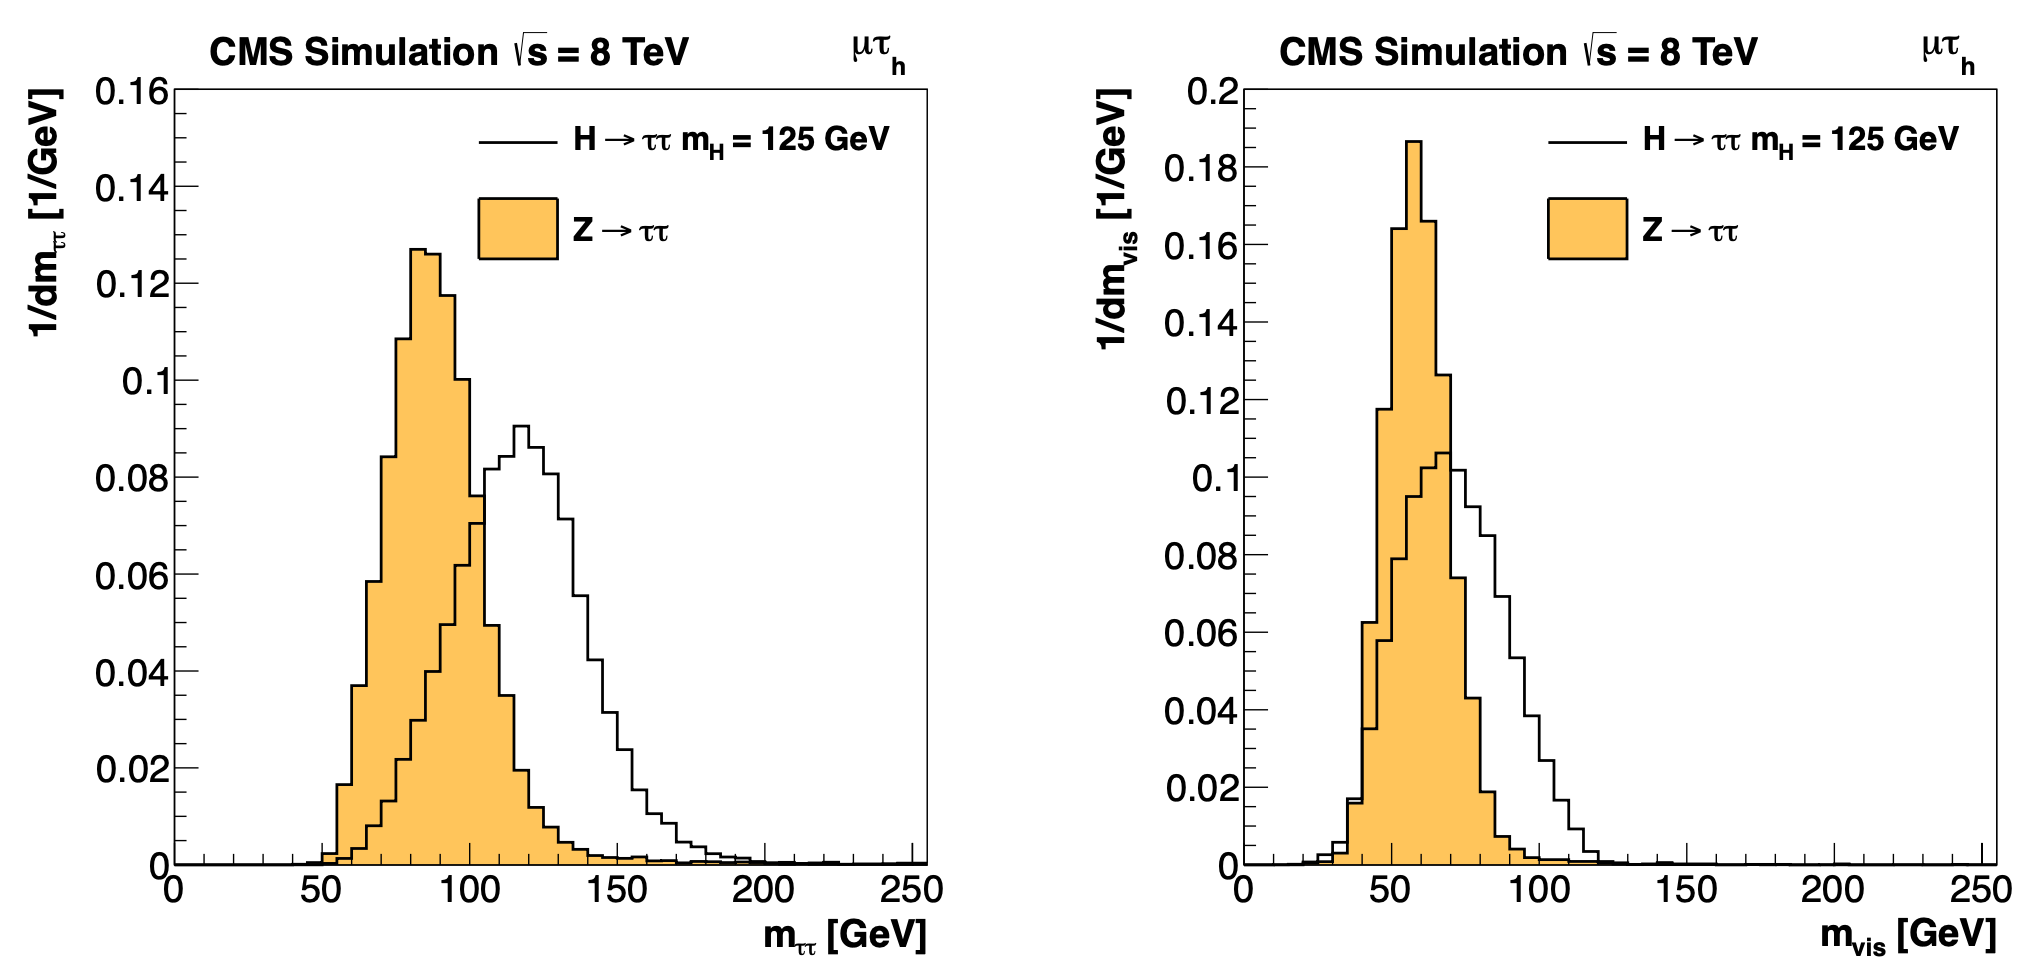
\includegraphics[width=15cm]{figures/ch-5-object-reconstruction-and-corrections-applied/original_SVFit_resolution_2014_SVFit_Bianchini.png}
    \caption[Distributions of $m_{\tau\tau}$ reconstructed by the classic SVFit algorithm, and masses of visible tau decay products (before SVFit).]{Distributions from \cite{2014_SVFit_Bianchini}, of $m_{\tau\tau}$ after reconstruction with the original SVFit algorithm (\textit{left}), and before SVFit with only the visible tau decay products (\textit{right}), for $H \rightarrow \tau\tau$ signal events of mass $m_H = 125$ GeV (\textit{black line}) and the $Z/\gamma^* \rightarrow \tau\tau$ background (\textit{orange, solid}), in the decay channel $\tau\tau \rightarrow \mu\tau_{h}$.} 
    \label{fig:classic_svfit_resolution}
\end{figure}


\subsection{FastMTT: optimized SVFit}
FastMTT \cite{CMS-AN-19-032-FastMTT} is a further simplification to the matrix element method of Classic SVFit which has comparable performance but is about 100 times faster. FastMTT drops the matrix element component of the computation without significant impact on the final mass resolution, and simplifies the computation of the transfer functions. The opening angle of the $\tau$ decay products with respect to the initial $\tau$ momenta approaches 0 for $\tau$ with high $\gamma = E_{\tau}/m_{\tau}$, with typical $\tau$ decays from the Z boson decays already satisfying this condition. In this collinear approximation, the dimensionality of the transfer function can be reduced in the computation of FastMTT, while still yielding similar results to Classic SVFit \cite{CMS-AN-19-032-FastMTT}. 


As the modeling of the CMS detector and underlying physics processes are imperfect, scale factors and corrections are applied to Monte Carlo events and in some cases, the embedded samples, to improve agreement with measurements in data. For the standard reconstruction physics objects in this work, central recommendations provided by dedicated physics object groups (POGs) in CMS are used.

Uncertainties in scale factors and corrections are also sources of systematic errors in the analysis, detailed in Chapter \ref{chapter:ch-8:systematic-uncertainties}. Systematic uncertainties in the tau, muon, and electron energy scales can shift the $p_{T}$ of the leptons up or down, causing a migration of number of events that pass the offline $p_{T}$ thresholds described in the previous section.



\section{Corrections applied to simulation and embedded}

\subsection{Tau energy scale}
\label{sec:tau_energy_scale}

An energy scale is applied to the transverse momentum $p_{T}$ and mass of the hadronic tau $\tau_{h}$ in the $\mu\tau_{h}$ and $e\tau_{h}$ channels, to correct for a deviation of the average reconstructed $\tau_{h}$ energy from the generator-level energy of the visible $\tau_{h}$ decay products. These correction factors are derived centrally \cite{CMS-TAU-16-003}, by fitting to events in $e\tau_{h}$ and $\mu\tau_{h}$ final states in $Z/\gamma^*$ events separately for the $h^\pm$, $h^\pm \pi^0$, and $h^\pm h^\mp h^\pm$ decays. The values used are shown in Table \ref{table:tau-ES}.

When applying the energy scale to the $\tau_{h}$, the 4-momentum of the missing transverse energy (MET) is adjusted such that the total 4-momenta of the $\tau_{h}$ and the MET remains unchanged \cite{twiki_TAU_POG_tauidrecommendationforrun2}.

\begin{table}[ht]
    \centering
    \begin{tabular}{|c|c|c|c|c|}
    \hline
    \multicolumn{5}{|c|}{Tau energy scale factor}                                   \\ \hline
    \hline
    Decay mode      & 2018              & 2017              & 2016 pre-VFP      & 2016 post-VFP     \\ \hline
    0               & 0.991 $\pm$ 0.008 & 0.986 $\pm$ 0.009 & 0.987 $\pm$ 0.01  & 0.993 $\pm$ 0.009 \\
    1               & 1.004 $\pm$ 0.006 & 0.999 $\pm$ 0.006 & 0.998 $\pm$ 0.006 & 0.991 $\pm$ 0.007 \\
    10              & 0.998 $\pm$ 0.007 & 0.999 $\pm$ 0.007 & 0.984 $\pm$ 0.008 & 1.001 $\pm$ 0.007 \\
    11              & 1.004 $\pm$ 0.009 & 0.996 $\pm$ 0.01  & 0.999 $\pm$ 0.011 & 0.997 $\pm$ 0.016 \\ \hline
    \end{tabular}
    \caption{Energy scales applied to genuine hadronic tau decays $\tau_{h}$ by data-taking year/era and decay mode, along with systematic errors.}
    \label{table:tau-ES}
\end{table}

\subsection{Muon energy scale}
\label{sec:muon_energy_scale}

An energy scale is applied to the $p_{T}$ and mass of genuine muons from $\tau$ decays in the $e\mu$ and $\mu\tau_{h}$ channels \cite{twiki_MUON_POG_recommendation}. The applied values are the same for MC and embedded samples and are shown in Table \ref{table:muon-ES}. Following the SM $H \rightarrow \tau\tau$ analysis, Rochester corrections are not applied, and instead prescriptions from \cite{twiki_MUO_simplified_ES} are followed.


\begin{table}[ht]
    \centering
    \begin{tabular}{|c|c|}
    \hline
    \multicolumn{2}{|c|}{Muon energy scale factor}      \\ \hline
    \hline
    Eta range                & Value for all years \\ \hline
    $|\eta| \in [0.0, 1.2)$  & 1.0 $\pm$ 0.004 \\
    $|\eta| \in [1.2, 2.1)$  & 1.0 $\pm$ 0.009 \\
    $|\eta| \in [2.1, 2.4)$  & 1.0 $\pm$ 0.027 \\
    \hline
    \end{tabular}
    \caption[Energy scales and systematic errors applied to genuine muons.]{Energy scales and systematic errors applied to genuine muons. The values are the same for MC and embedded for all years \cite{twiki_HiggsToTauTauWorkingLegacyRun2} \cite{twiki_MUO_simplified_ES}.}
    \label{table:muon-ES}
\end{table}


\subsection{Electron energy scale}
\label{sec:electron_energy_scale}

Corrections to the electron energy scale are applied to genuine $e$ from $\tau$ decays, and are binned in two dimensions by electron $p_{T}$ and $\eta$ for barrel vs. endcap \cite{twiki_Electron_POG_recommendation}. The scale factors are binned in $p_{T}$ and $\eta$ for MC samples: e.g. values for 2018 are shown in Fig. \ref{fig:egamma-POG-UL-egamma-scale-factors} from \cite{twiki_Electron_UL_2016_2017_2018}. For embedded samples the electron energy scale is taken as only binned in $\eta$ (Table \ref{table:ele-ES-embedded}).

% https://twiki.cern.ch/twiki/pub/CMS/EgammaUL2016To2018/egammaEffi.txt_Ele_wp90noiso_egammaPlots.pdf
\begin{figure}[h]
    \centering
    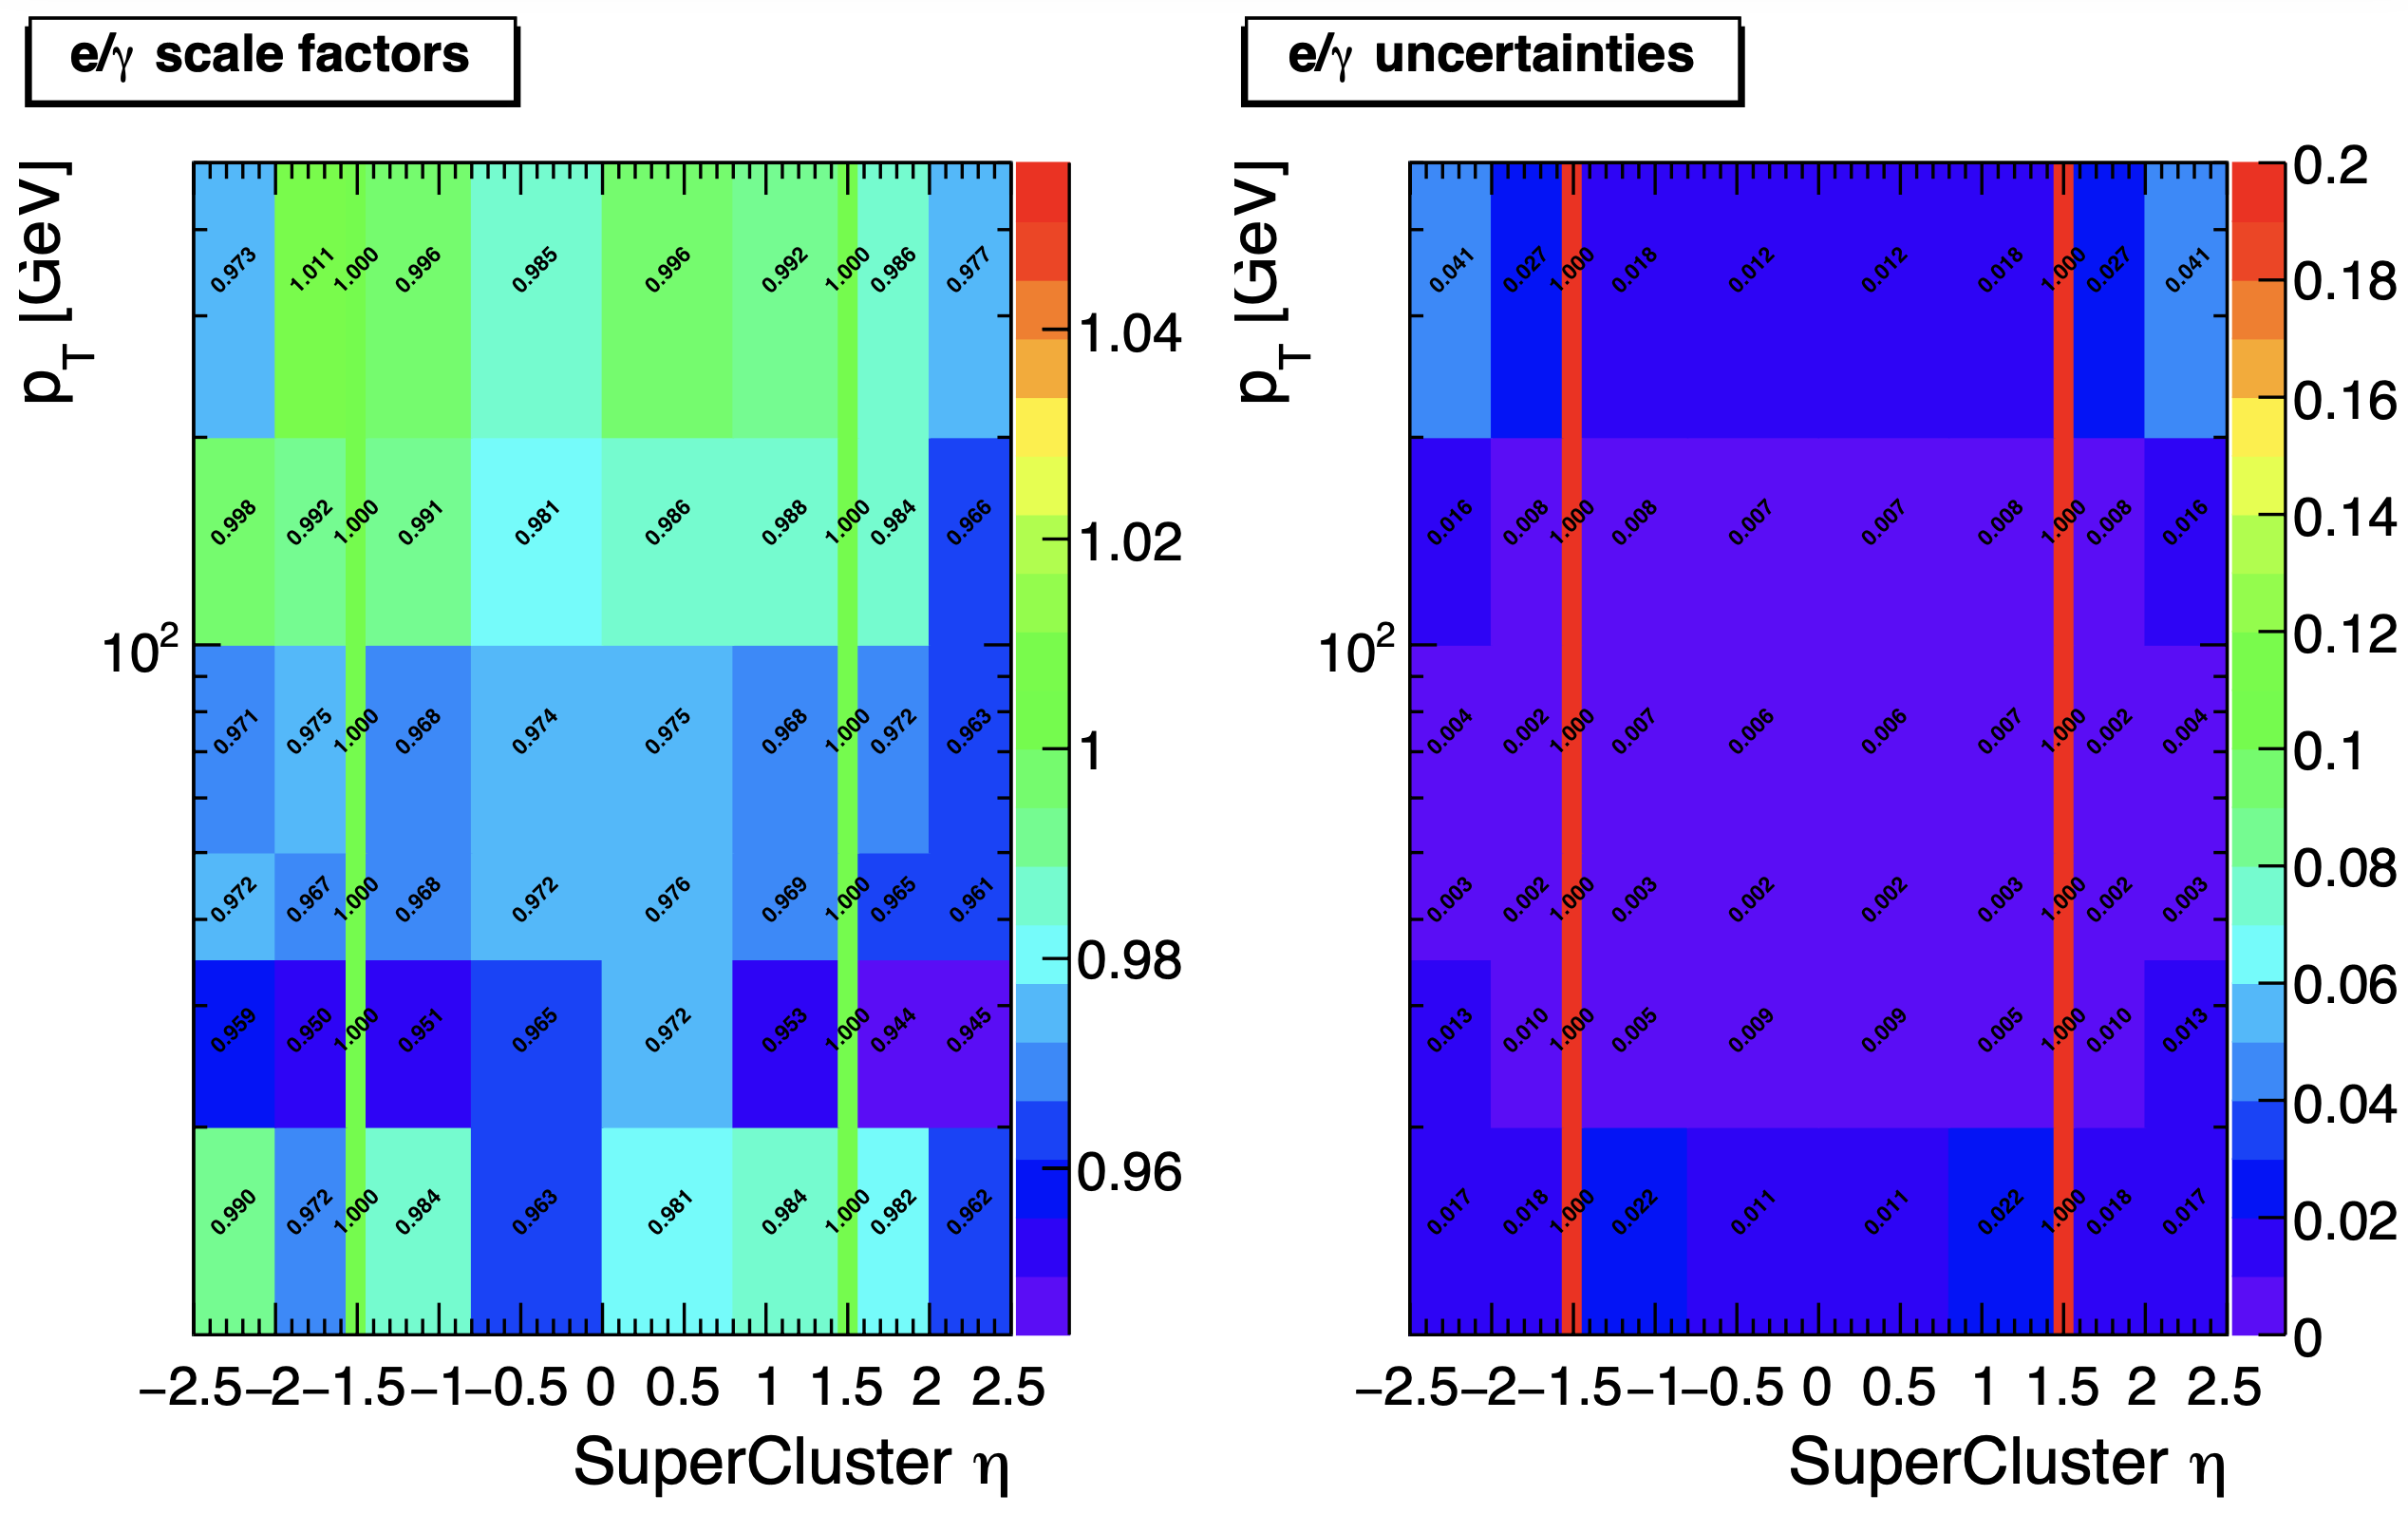
\includegraphics[width=15cm]{figures/ch-5-object-reconstruction-and-corrections-applied/egamma-POG-UL-egamma-scale-factors.png}
    \caption[Electron/photon energy scale factors and uncertainties for 2018.]{Electron/photon energy scale factors (\textit{left}) and corresponding uncertainties (\textit{right}) binned in the electron $\eta$ and $p_{T}$, for the data-taking year 2018 \cite{twiki_Electron_UL_2016_2017_2018}.} 
    \label{fig:egamma-POG-UL-egamma-scale-factors}
\end{figure}


\begin{table}[h]
    \centering
    \begin{tabular}{|c|c|c|c|}
    \hline
    \multicolumn{4}{|c|}{Electron energy scale factor for embedded samples}                                   \\ \hline
    \hline
    Eta range                   & 2018               & 2017               & 2016     \\ \hline
    $|\eta| \in [0.0, 1.479)$   & 0.973 $\pm$ 0.005  & 0.986 $\pm$ 0.009  & 0.9976 $\pm$ 0.0050 \\
    $|\eta| \in [1.479, 2.4)$   & 0.980 $\pm$ 0.0125 & 0.887 $\pm$ 0.0125 & 0.993 $\pm$ 0.0125 \\ \hline
    \end{tabular}
    \caption[Energy scales and systematic errors applied to electrons in embedded samples by data-taking year/era.]{Energy scales and systematic errors applied to electrons in embedded samples, binned in the electron $\eta$, by data-taking year \cite{twiki_embedded_preUL_2016} \cite{twiki_embedded_preUL_2017} \cite{twiki_embedded_preUL_2018}.}
    \label{table:ele-ES-embedded}
\end{table}

\subsection{$\tau_{h}$ identification efficiency}
\label{sec:tauh_id_efficiency}

The $\tau_{h}$ identification efficiency can differ in data and MC \cite{twiki_TAU_POG_tauidrecommendationforrun2}. Recommended corrections are provided by the Tau POG, and we use the medium DeepTau vs. jet working point values. The identification efficiency is measured in $Z \rightarrow \tau\tau$ events in the $\mu\tau_{h}$ final state, and is binned in $p_{T}$ due to clear $p_{T}$ dependence of the DeepTau ID. 


\begin{table}[h]
    \centering
    \begin{tabular}{|c|c|c|c|c|c|c|}
    \hline
    \multicolumn{7}{|c|}{Tau ID efficiency for DeepTau Medium vs. jet WP in 2018}                                   \\ \hline
    \hline
    $p_{T}$ (GeV)  & $<20$  & $(20, 25]$ & $(25, 30]$ & $(30, 35]$ & $(35, 40]$ & $(40, 500] $   \\ \hline
    Central value  & 0      & 0.945      & 0.946      & 0.916      & 0.921      & 1.005 \\
    Up value       & 0      & 1.001      & 0.981      & 0.946      & 0.950      & 1.035 \\
    Down value     & 0      & 0.888      & 0.981      & 0.883      & 0.893      & 0.953 \\ \hline
    \end{tabular}
    \caption[Tau ID efficiency for the DeepTau vs. jet medium working point, with central, up, and down values for 2018, binned in the tau $p_{T}$.]{Tau ID efficiency for the DeepTau vs. jet medium working point, with central, up, and down values for 2018, binned in the tau $p_{T}$ \cite{twiki_TAU_POG_tauidrecommendationforrun2}.}
    \label{table:tauIDeff_deepTau_vs_jet_medium_WP}
\end{table}


\subsection{Trigger efficiencies}

Scale factors are applied to correct for differences in trigger efficiencies between MC and embedded vs. data, with values taken from tools provided by the Standard Model $H \rightarrow \tau\tau$ working group which uses the same trigger paths \cite{twiki_HiggsToTauTauWorkingLegacyRun2}. In the following sections we review relevant trigger efficiencies in data, which form the basis of the trigger efficiency corrections applied to MC and embedded.

\subsection{Tau trigger efficiencies}
The efficiencies in data of the single-$\tau_{h}$ leg in $\mu\tau_{h}$, $e\tau_{h}$, and di-$\tau_{h}$ triggers is computed centrally per using a Tag and Probe (TnP) method \cite{CMS-DP-2019-012} which is outlined here. In this method, $Z \rightarrow \tau\tau \rightarrow \mu\tau_{h}$ are selected in data and a Drell-Yan simulated sample ($Z \rightarrow \ell\ell, \ell = e, \mu, \tau_{h}$) with high purity. Cuts are applied to reject events not in this final state, e.g. suppressing $Z \rightarrow \mu\mu$ by vetoing events with a single loose ID muon. An isolated muon candidate (the tag) with online $p_{T} > 27$ GeV and $|\eta| < 2.1$ is identified and matched to an offline $\mu$. An offline $\tau_{h}$ candidate (the probe) is selected, which is separated from the tag $\mu$, and has $p_{T} > 20$ GeV and $|\eta| < 2.1$. The probe $\tau_{h}$ must pass anti-muon and anti-electron discriminators to avoid fakes from muons and electrons, and must pass the medium MVA tau isolation to suppress fakes from QCD jets. The trigger efficiency in the TnP method is calculated as 
\begin{equation}
    \text{Efficiency} = \frac{\text{Number of events passing the TnP selection with fires the HLT path}}{\text{Number of events passing the TnP selection}}
\end{equation}


The efficiencies for the hadronic tau legs in the relevant channels of this analyses ($\mu\tau_{h}$ and $e\tau_{h}$) as a function of the offline tau $p_{T}$ and $\eta$, are shown for data taken in 2016, 2017, and 2018 in Figures \ref{fig:mutauEfficiencyPt_eachYear_mediumTauMVA_Data} and \ref{fig:etauEfficiencyPt_eachYear_mediumTauMVA_Data} \cite{CMS-DP-2019-012} \cite{twiki_Tau_Lepton_Run_2_trigger_performance}. In both figures, the different HLT thresholds and differences in the L1 seed result in higher efficiencies in 2016 and differences in shapes of the 2016 efficiencies compared to 2017 and 2018. The low pileup in 2016 also leads to higher efficiencies in that year.


\begin{figure}[h]
    \centering
    \begin{subfigure}{0.45\textwidth}
        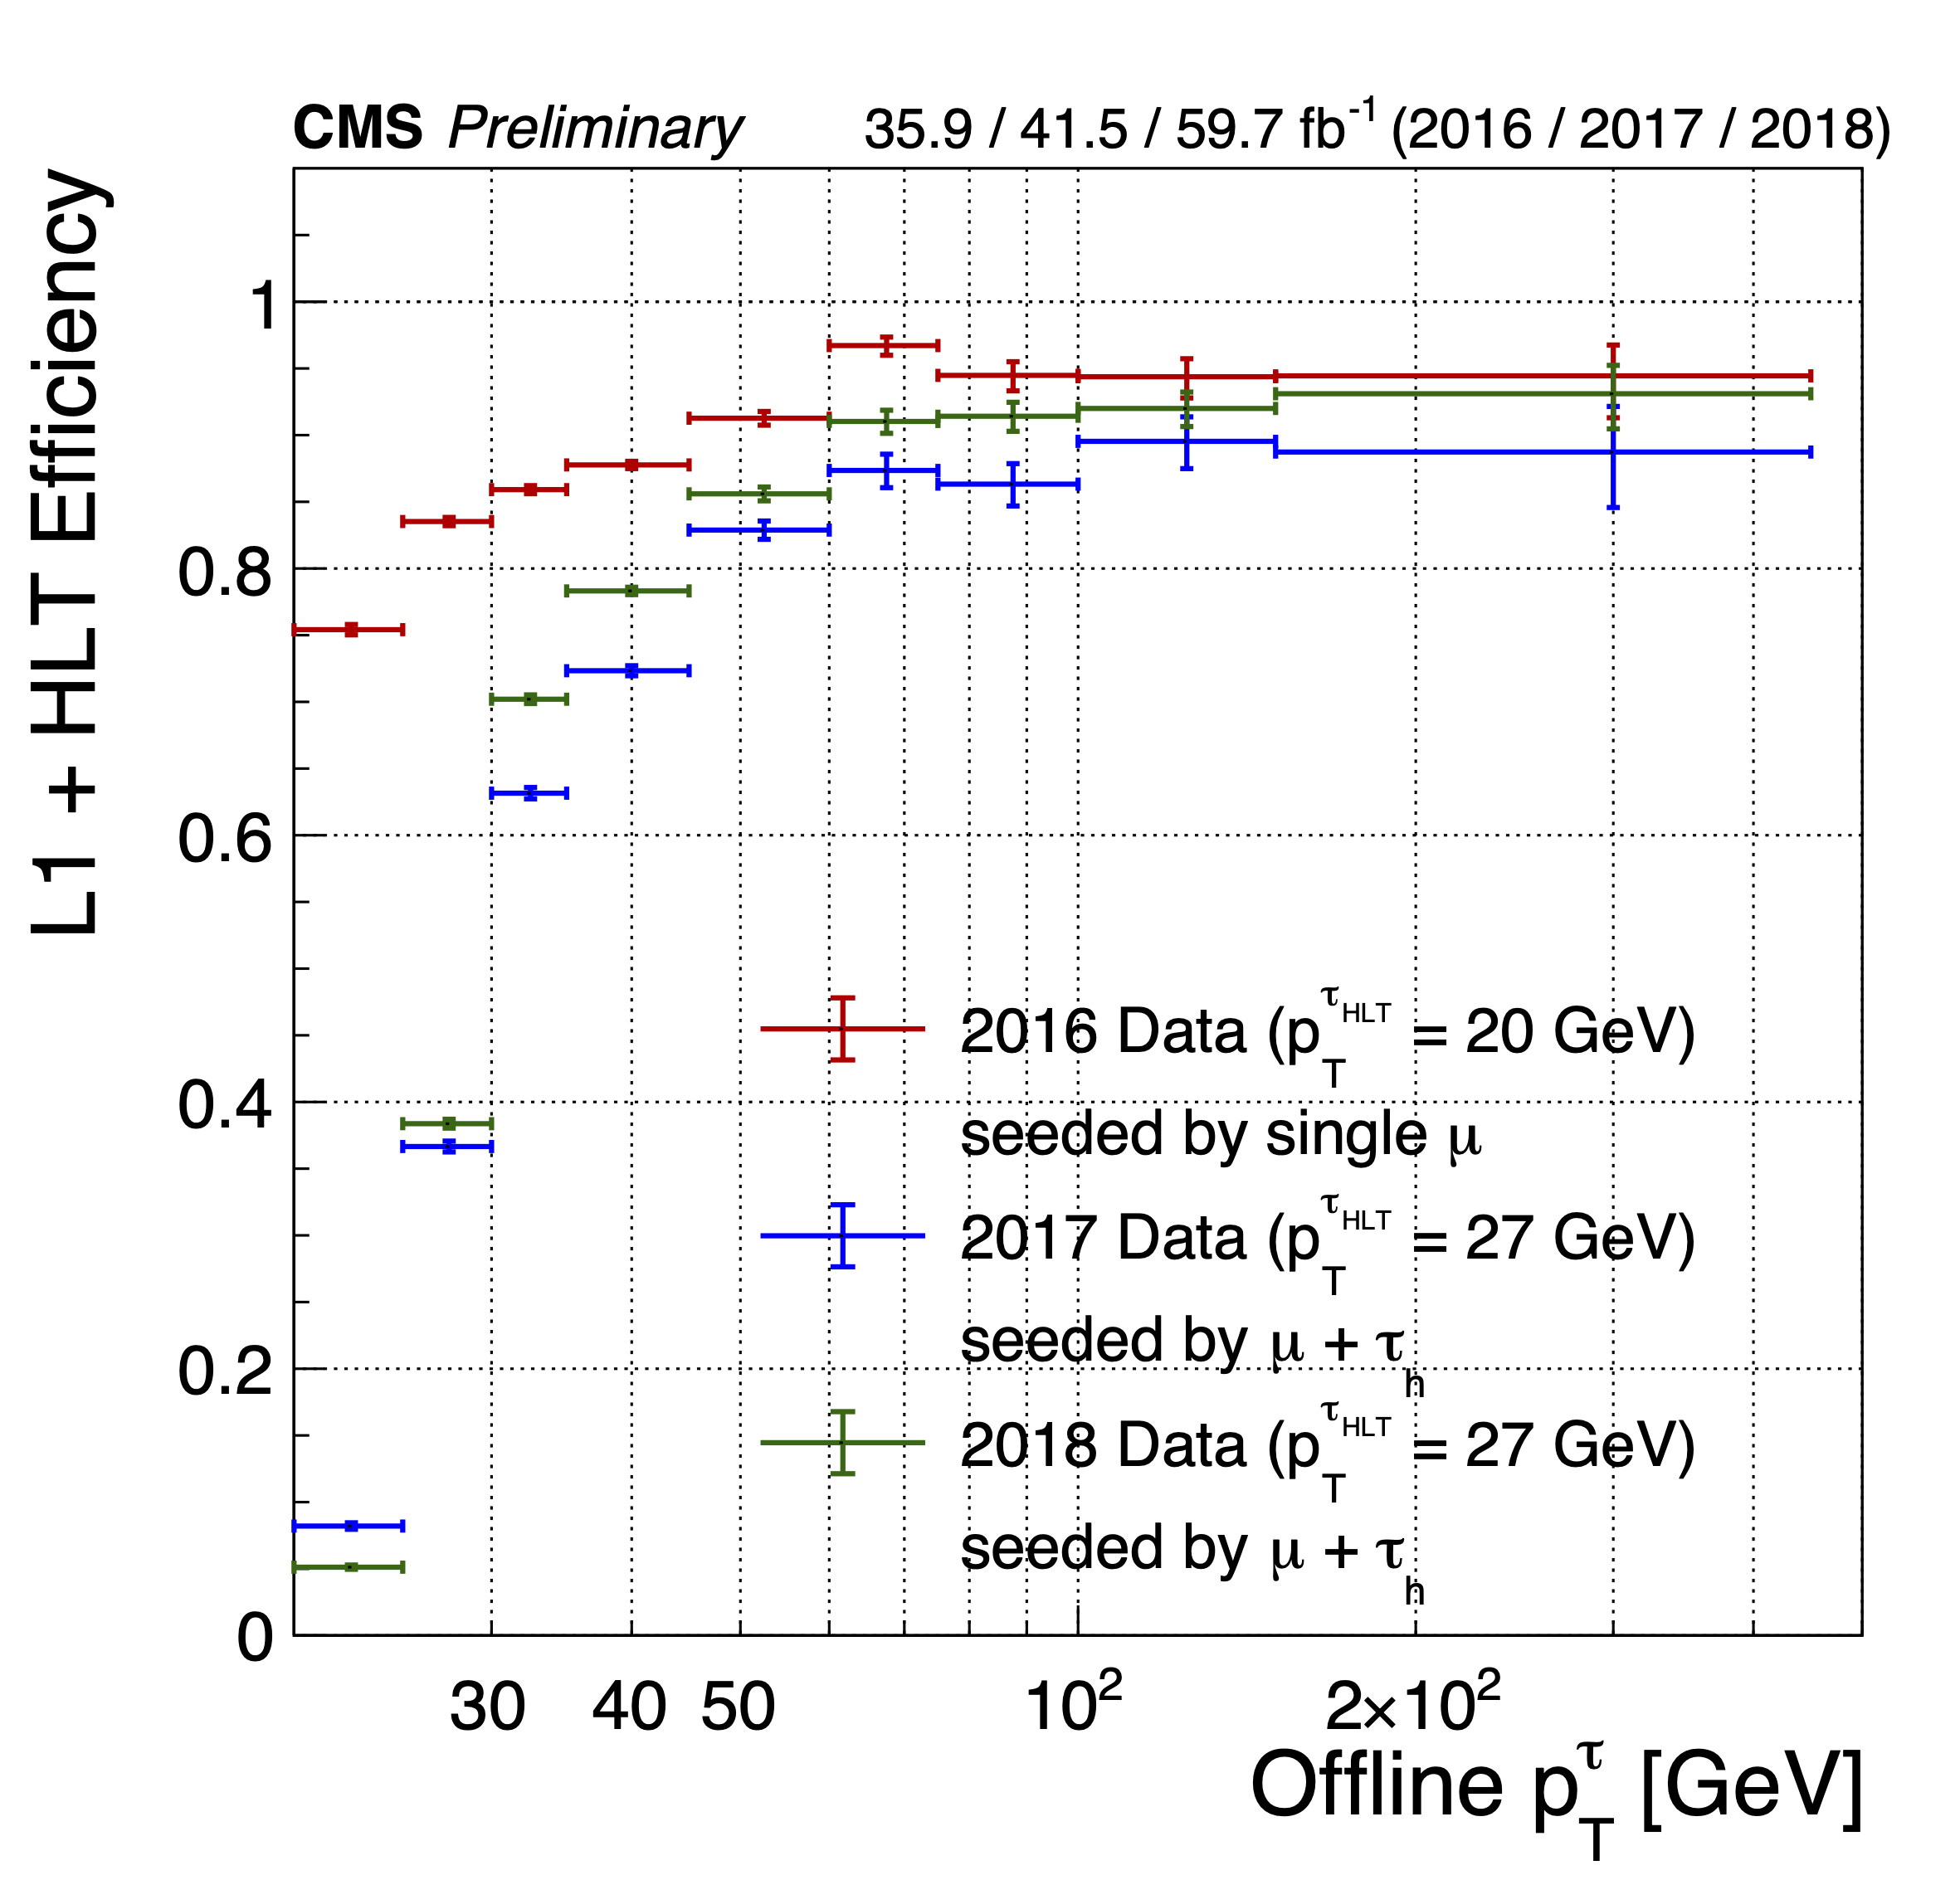
\includegraphics[width=1.0\textwidth]{figures/ch-5-object-reconstruction-and-corrections-applied/mutauEfficiencyPt_eachYear_mediumTauMVA_Data.png}
        \caption{$\tau_{h}$ efficiency from $\mu\tau_{h}$ trigger.}
        \label{fig:mutauEfficiencyPt_eachYear_mediumTauMVA_Data}
    \end{subfigure}
    \hfill
    \begin{subfigure}{0.45\textwidth}
        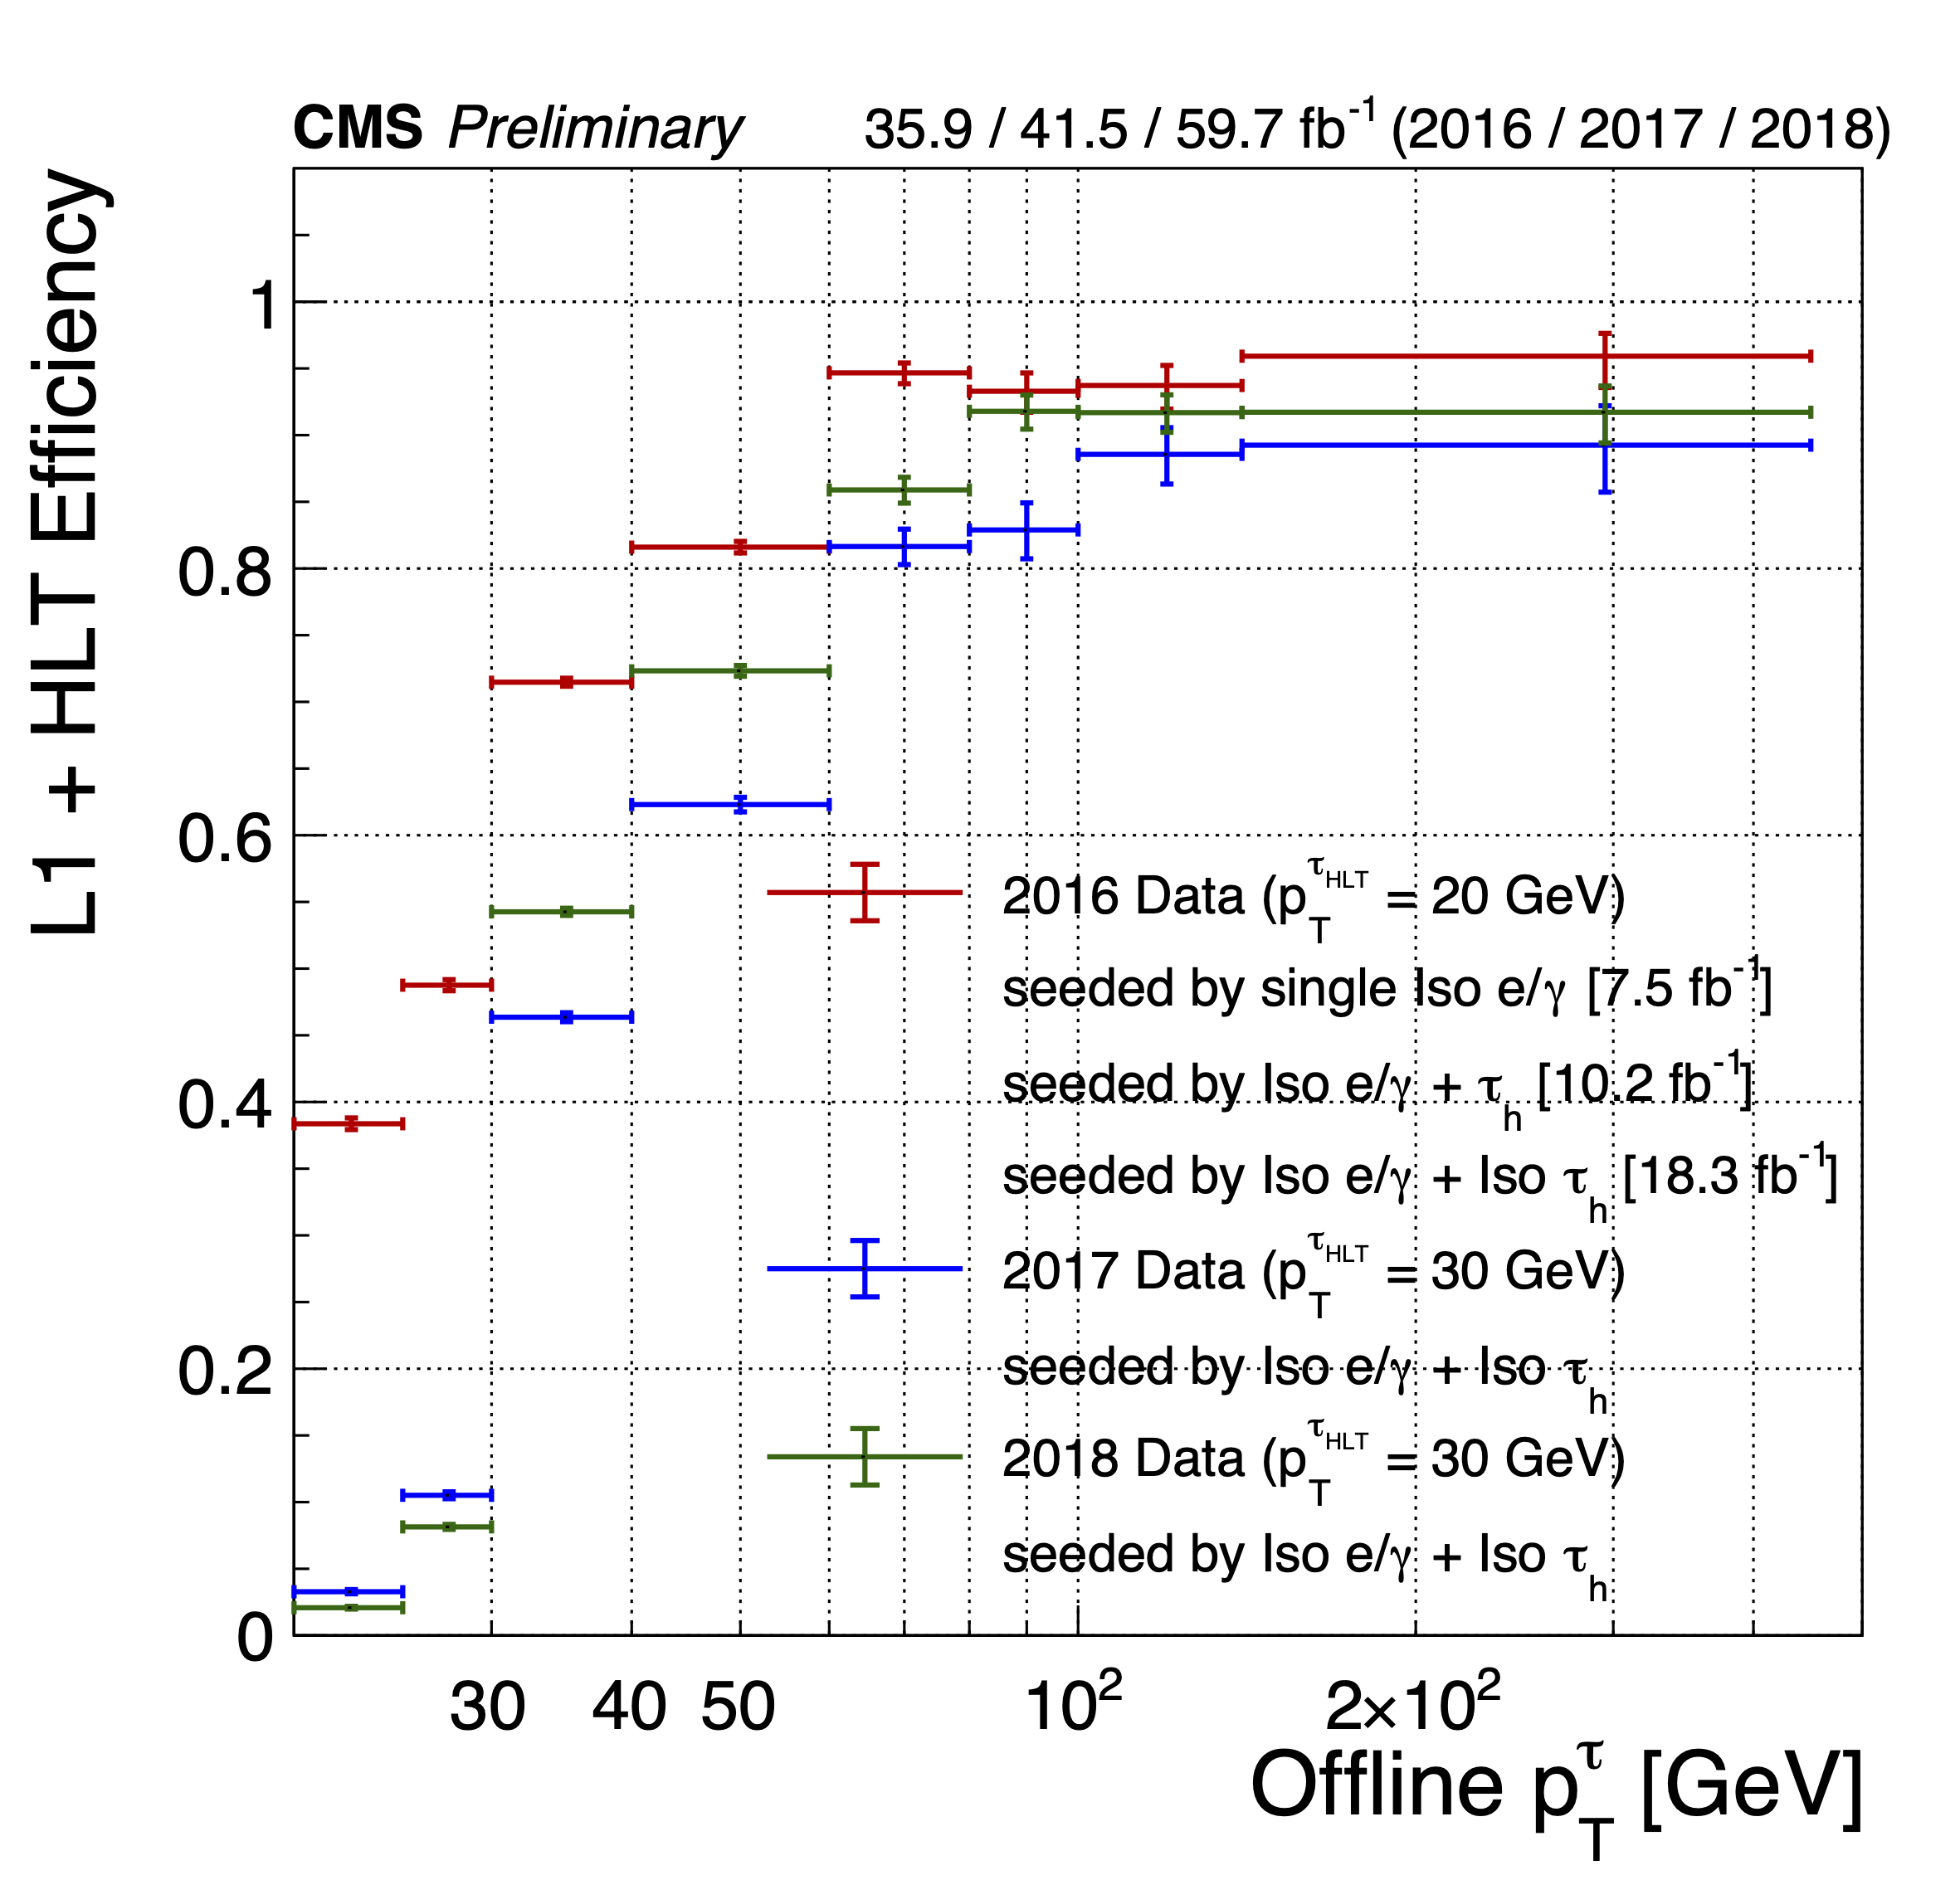
\includegraphics[width=1.0\textwidth]{figures/ch-5-object-reconstruction-and-corrections-applied/etauEfficiencyPt_eachYear_mediumTauMVA_Data.png}
        \caption{$\tau_{h}$ efficiency from $e\tau_{h}$ trigger.}
        \label{fig:etauEfficiencyPt_eachYear_mediumTauMVA_Data}
    \end{subfigure}
    \caption[Hadronic tau leg efficiency of the cross-triggers for $\mu\tau_{h}$ (\textit{left}) and $e\tau_{h}$ (\textit{right}) triggers as a function of offline tau $p_{T}$ for 2016, 2017, and 2018.]{Hadronic tau leg efficiency of the cross-triggers for $\mu\tau_{h}$ (\textit{left}) and $e\tau_{h}$ (\textit{right}) triggers as a function of offline tau $p_{T}$ for the years 2016 (\textit{red}), 2017 (\textit{blue}) and 2018 (\textit{green}), from \cite{twiki_Tau_Lepton_Run_2_trigger_performance}. HLT $p_{T}$ thresholds and L1 seeds are indicated in the legends.} 
\end{figure}


\subsection{Single muon trigger efficiencies}
The efficiencies for the single isolated muon trigger with $p_{T} > 24$ GeV used in this analysis, is shown for the data-taking year 2018 in Fig. \ref{fig:single_muon_24GeV_efficiency_vs_pt} as a function of the muon $p_{T}$ and as a function of the muon $|\eta|$ in Fig. \ref{fig:single_muon_24GeV_efficiency_vs_eta} from \cite{CMS-DP-2018-034}. The data is split with respect to a HLT muon reconstruction update that was deployed on 15/05/2018. A small asymmetry in efficiencies between negative and positive $\eta$ in Fig. \ref{fig:single_muon_24GeV_efficiency_vs_eta} is due to disabled muon chambers (CSCs). The efficiencies shown are estimated using a Tag and Probe method using $Z\rightarrow \mu\mu$ events, with the tag being an offline muon with $p_{T} > 29$ GeV and $|\eta| < 2.4$ passing a tight ID criteria, and the probe is an online (L1) trigger object with $\Delta R < 0.3$ and passing tight ID and Particle Flow based isolation requirements with $p_{T} > 26$ GeV.

\begin{figure}[h]
    \centering
    \begin{subfigure}{0.45\textwidth}
        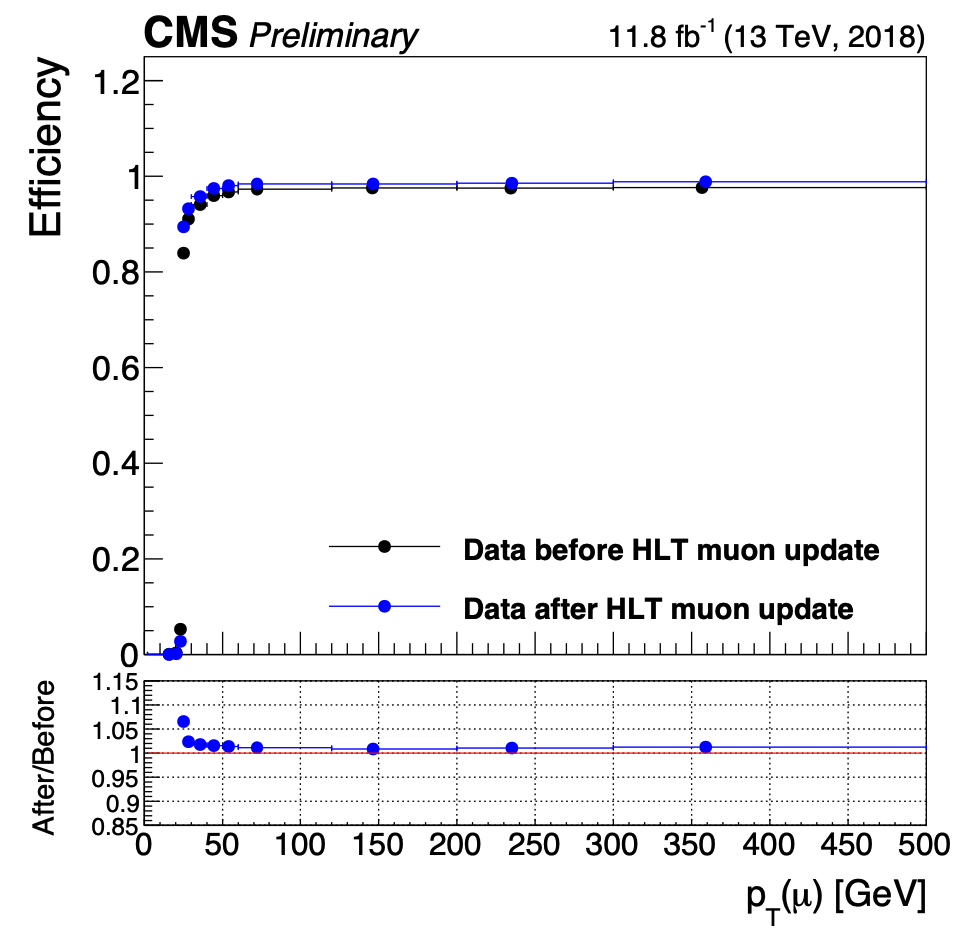
\includegraphics[width=1.0\textwidth]{figures/ch-5-object-reconstruction-and-corrections-applied/singleMuon_isolated_efficiency_vs_pt}
        \caption{Muon efficiency vs $p_{T}$ for SingleMuon.}
        \label{fig:single_muon_24GeV_efficiency_vs_pt}
    \end{subfigure}
    \hfill
    \begin{subfigure}{0.45\textwidth}
        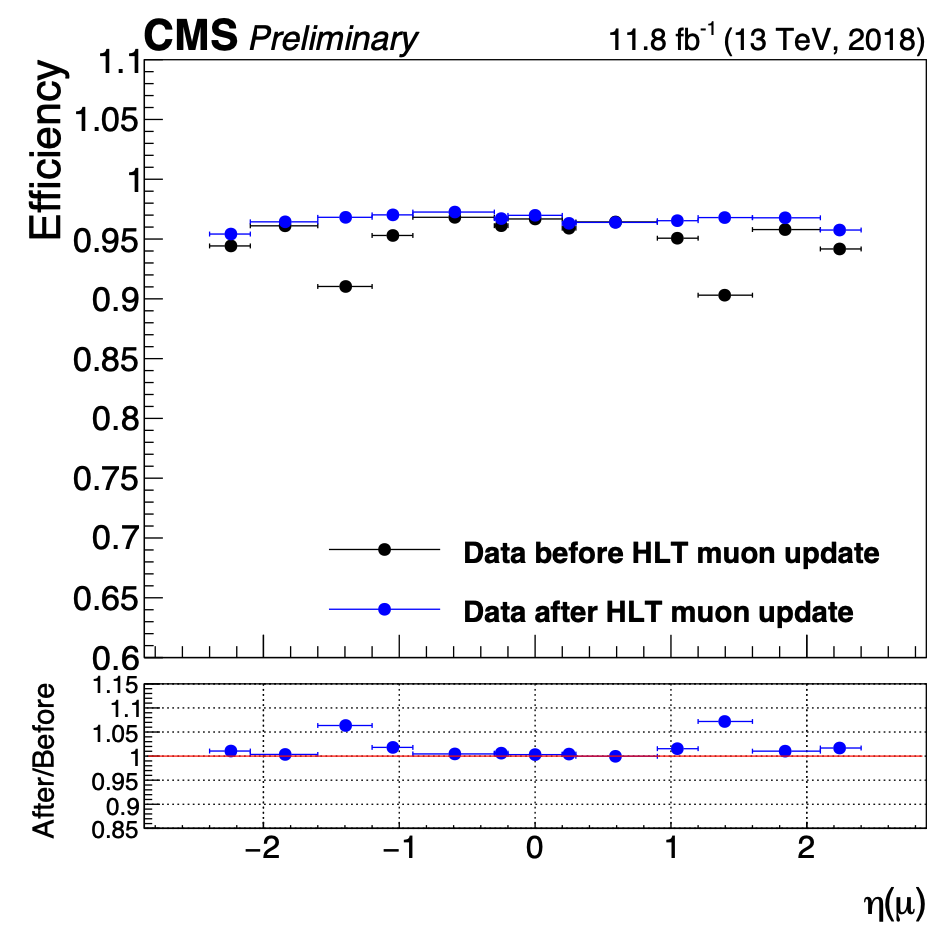
\includegraphics[width=1.0\textwidth]{figures/ch-5-object-reconstruction-and-corrections-applied/singleMuon_isolated_efficiency_vs_eta}
        \caption{Muon efficiency vs $|\eta|$ for SingleMuon.}
        \label{fig:single_muon_24GeV_efficiency_vs_eta}
    \end{subfigure}
    \caption[Trigger efficiencies in data (\textit{top panels}) and ratio of efficiencies after/before a HLT muon reconstruction update (\textit{bottom panels}) for the muon in the isolated single muon trigger with threshold $p_{T} > 24$ GeV in the data-taking year 2018, as functions of the muon $p_{T}$ (\textit{left}) and muon $|\eta|$ (\textit{right}).]{Trigger efficiencies in data (\textit{top panels}) and ratio of efficiencies after/before a HLT muon reconstruction update (\textit{bottom panels}) for the muon in the isolated single muon trigger with threshold $p_{T} > 24$ GeV in the data-taking year 2018, as functions of the muon $p_{T}$ (\textit{left}) and muon $|\eta|$ (\textit{right}). Only statistical errors are shown \cite{CMS-DP-2018-034}.} 
\end{figure}

\subsection{Single electron trigger efficiencies}

The efficiencies in data, and the ratio between data and MC, of the single electron HLT trigger with $p_{T}$ threshold 32 GeV used in this analysis are shown for 2018, as a function of the electron $p_{T}$ in Fig. \ref{fig:single_ele_32GeV_efficiency_vs_pt} and of the electron $|\eta|$ in Fig. \ref{fig:single_ele_32GeV_efficiency_vs_eta}, from \cite{CMS-DP-2020-016}. In the Tag and Probe method used for the 2018 dataset, the tag is an offline reconstructed electron with $|\eta| \leq 2.1$ and not in the barrel and endcap overlap region, with $p_{T} > 35$ GeV with tight isolation and shower shape requirements, firing the tag trigger. The probe is an offline reconstructed electron with $|\eta| \leq 2.5$ with $E_T^\text{ECAL} > 5$ GeV with no extra identification criteria \cite{CMS-DP-2020-016}. 

The disagreement between data and MC, particularly at low transverse momentum, is in part due to detector effects that are difficult to simulate, such as crystal transparency losses in the ECAL and the evolution of dead regions in the pixel tracker \cite{CMS-DP-2020-016}.

\begin{figure}[h]
    \centering
    \begin{subfigure}{0.45\textwidth}
        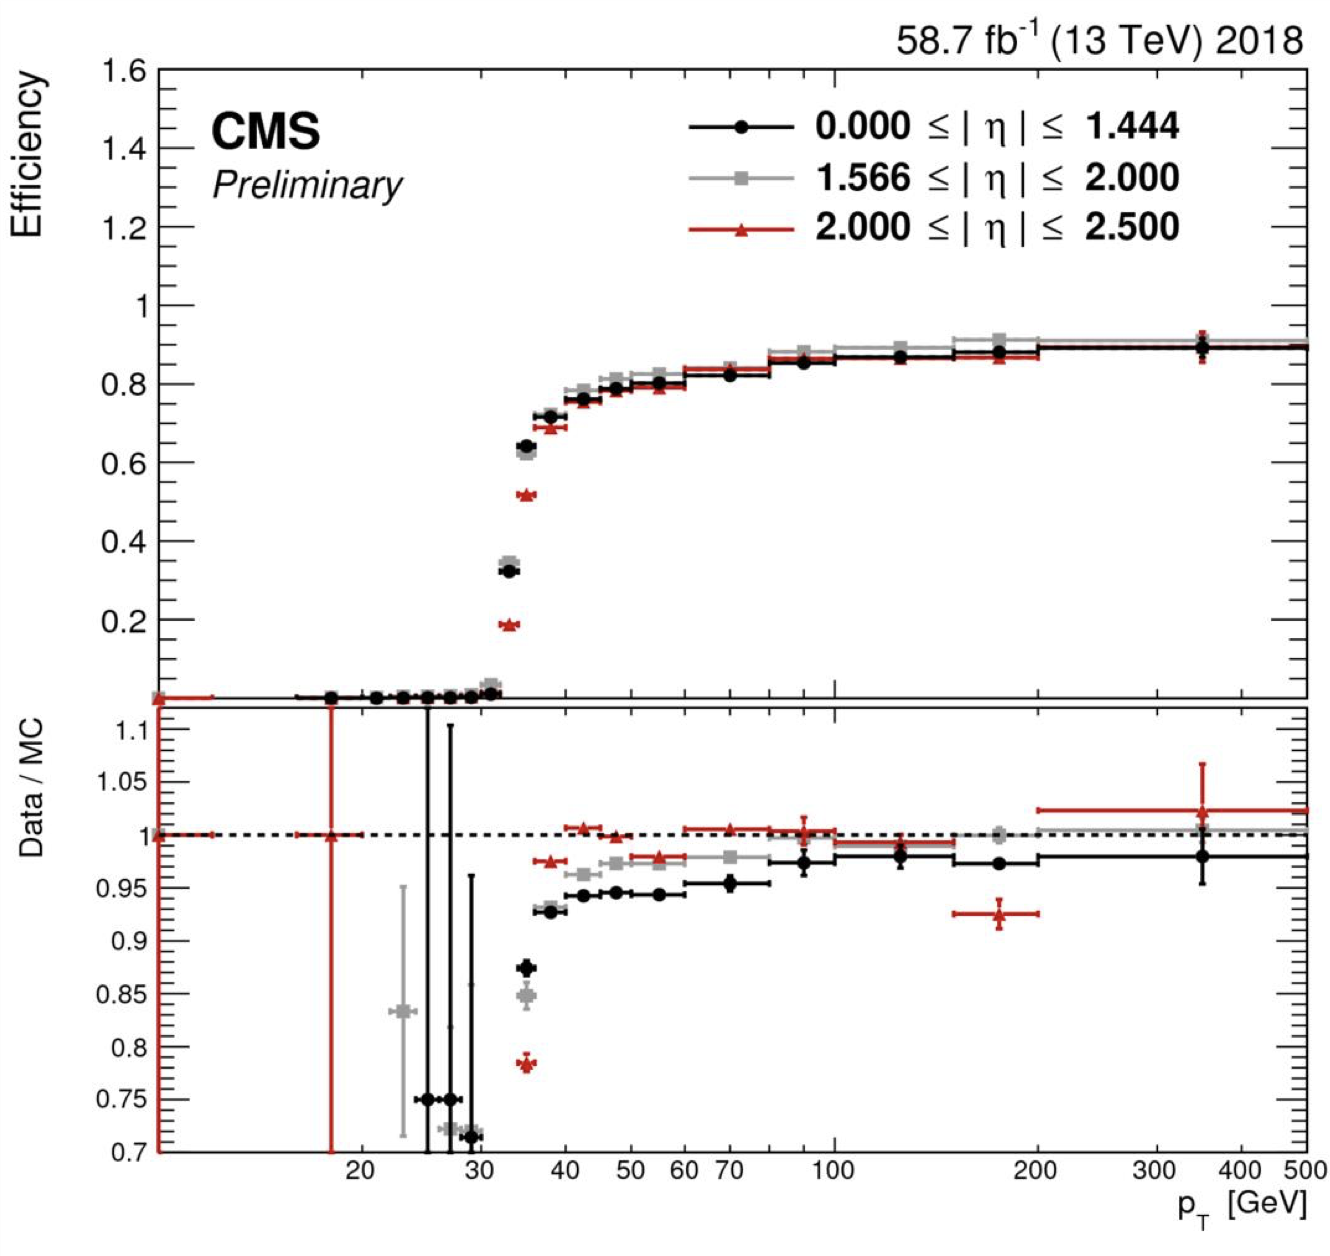
\includegraphics[width=1.0\textwidth]{figures/ch-5-object-reconstruction-and-corrections-applied/electron_Ele32_WPTight_Gsf_efficiency_vsPt}
        \caption{Electron efficiency vs $p_{T}$ for single electron.}
        \label{fig:single_ele_32GeV_efficiency_vs_pt}
    \end{subfigure}
    \hfill
    \begin{subfigure}{0.45\textwidth}
        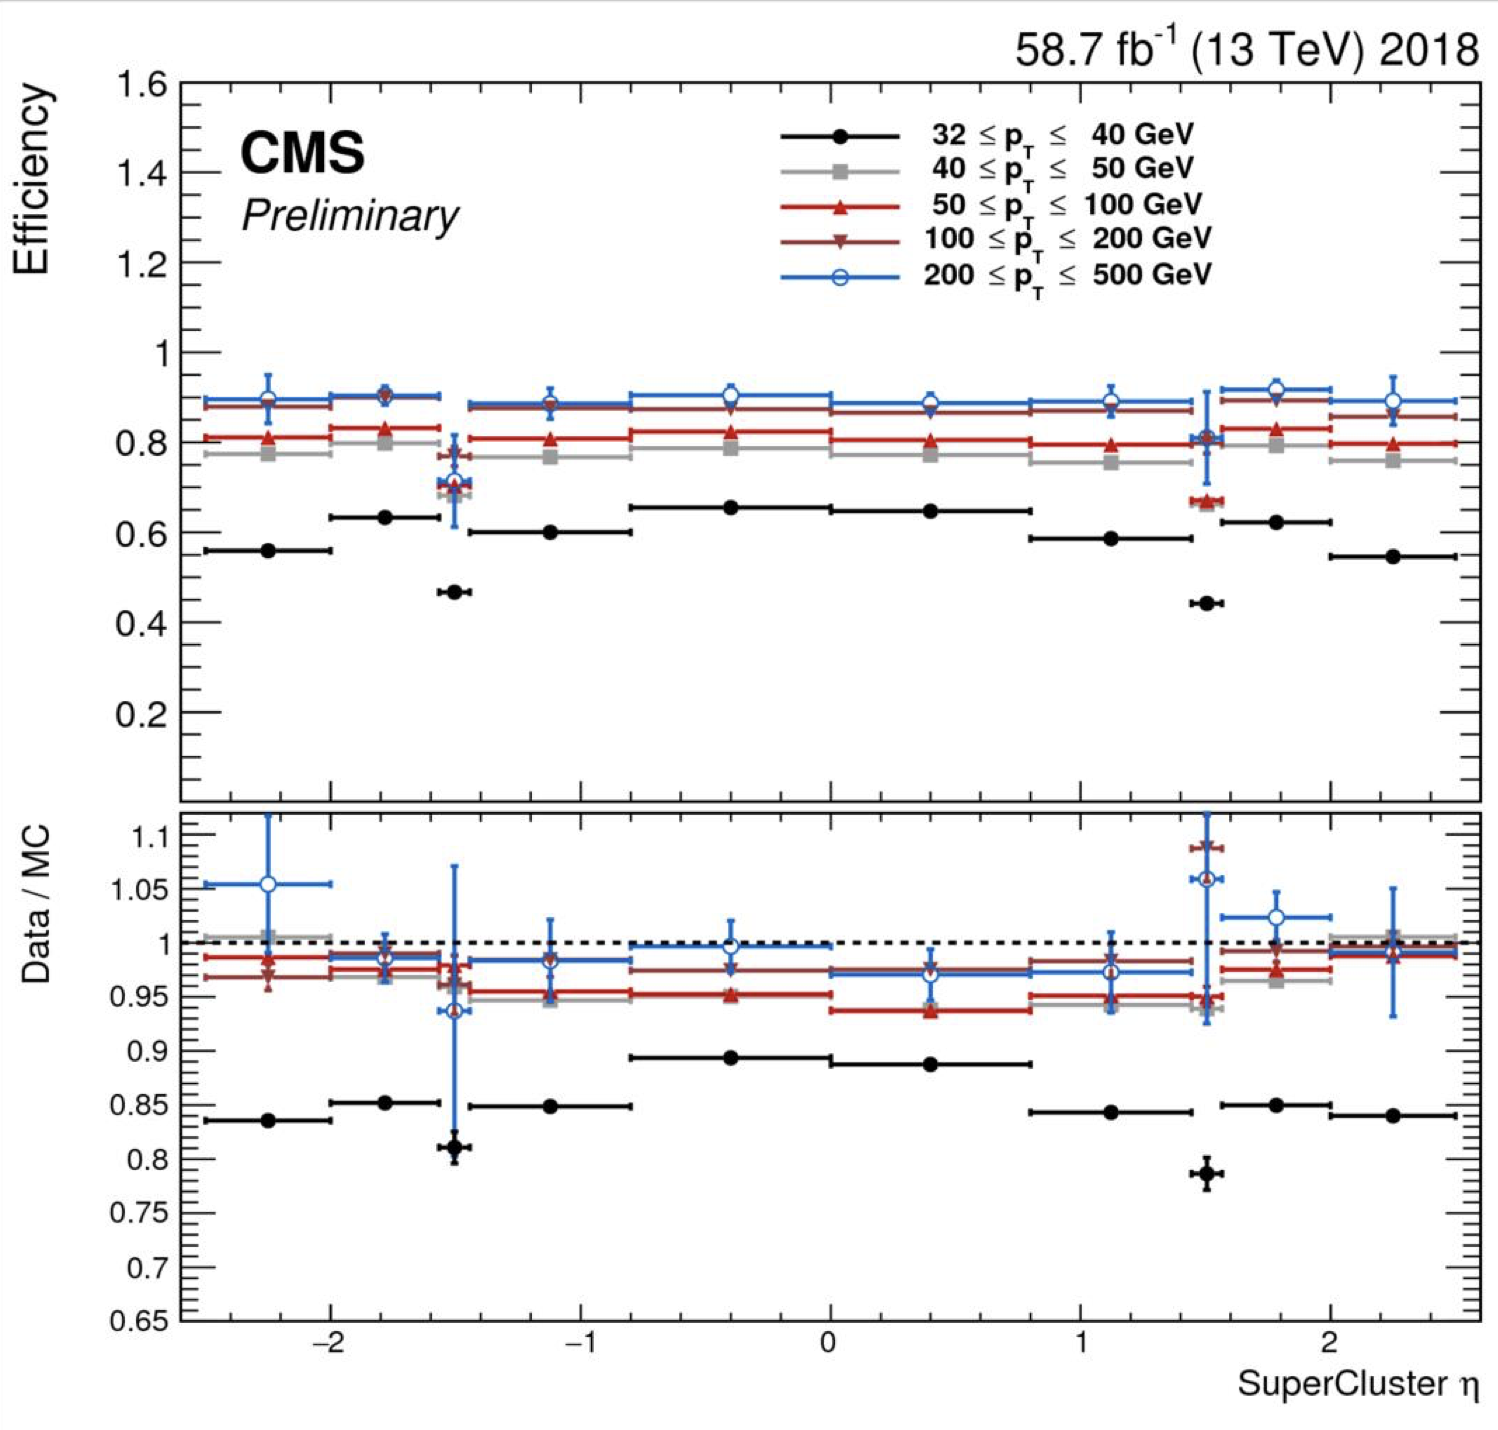
\includegraphics[width=1.0\textwidth]{figures/ch-5-object-reconstruction-and-corrections-applied/electron_Ele32_WPTight_Gsf_efficiency_vsEta}
        \caption{Electron efficiency vs $|\eta|$ for single electron.}
        \label{fig:single_ele_32GeV_efficiency_vs_eta}
    \end{subfigure}
    \caption[Trigger efficiencies in data and the data/MC ratio for the electron in the single electron trigger with threshold $p_{T} > 32$ GeV in the data-taking year 2018, as functions of the electron $p_{T}$ (\textit{left}) and electron $|\eta|$ (\textit{right}).]{Trigger efficiencies in data, and the data/MC ratio for the electron in the single electron trigger with threshold $p_{T} > 32$ GeV in the data-taking year 2018, as functions of the electron $p_{T}$ (\textit{left}) and electron $|\eta|$ (\textit{right}) \cite{CMS-DP-2020-016}. In the plot vs. $p_{T}$, the region 1.442 $\leq |\eta| \leq$ 1.566 is not included as it corresponds to the transition between barrel and endcap parts of the ECAL.} 
\end{figure}


\subsection{$e\mu$ cross-trigger efficiencies}

The efficiencies of the electron and muons for the cross-trigger with leading muon used in the $e\mu$ channel are shown for data in 2016, 2017, and 2018 in Figures \ref{fig:ele_efficiency_vs_pT_emu} and \ref{fig:muon_efficiency_vs_eta_emu} \cite{CMS-DP-2019-025}. These efficiencies were measured centrally using a Tag and Probe in events with $Z$ to dileptons with the same flavour and opposite charge, where the tags are an isolated muon or electron, and the probe (offline) candidate is required to satisfy the same lepton selection as that of the tag candidate, be matched within $\Delta R < 0.1$ with a corresponding online trigger object, and also to pass the cross-trigger. The trigger efficiency is then:
\begin{equation}
    \text{Efficiency} = \frac{\text{Events passing lepton pair selections and probe passing trigger}}{\text{Events passing lepton pair selections}}
\end{equation}

\begin{figure}[h]
    \centering
    \begin{subfigure}{0.45\textwidth}
        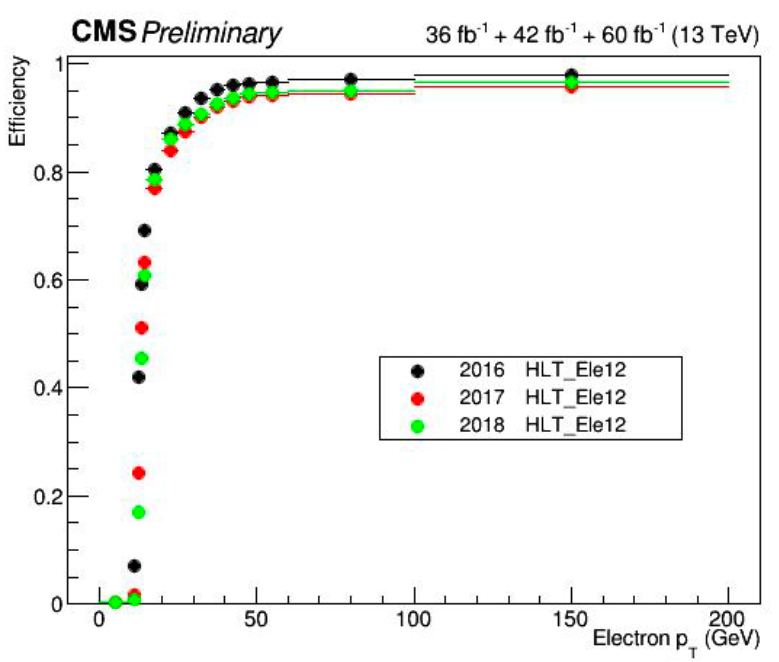
\includegraphics[width=1.0\textwidth]{figures/ch-5-object-reconstruction-and-corrections-applied/ele_efficiency_vs_pT_emu_HLT_Mu23_TrkIsoVVL_Ele12_CaloIdL_TrackIdL_IsoVL_DZ.png}
        \caption{Electron efficiency vs. $p_{T}$.}
        \label{fig:ele_efficiency_vs_pT_emu}
    \end{subfigure}
    \hfill
    \begin{subfigure}{0.45\textwidth}
        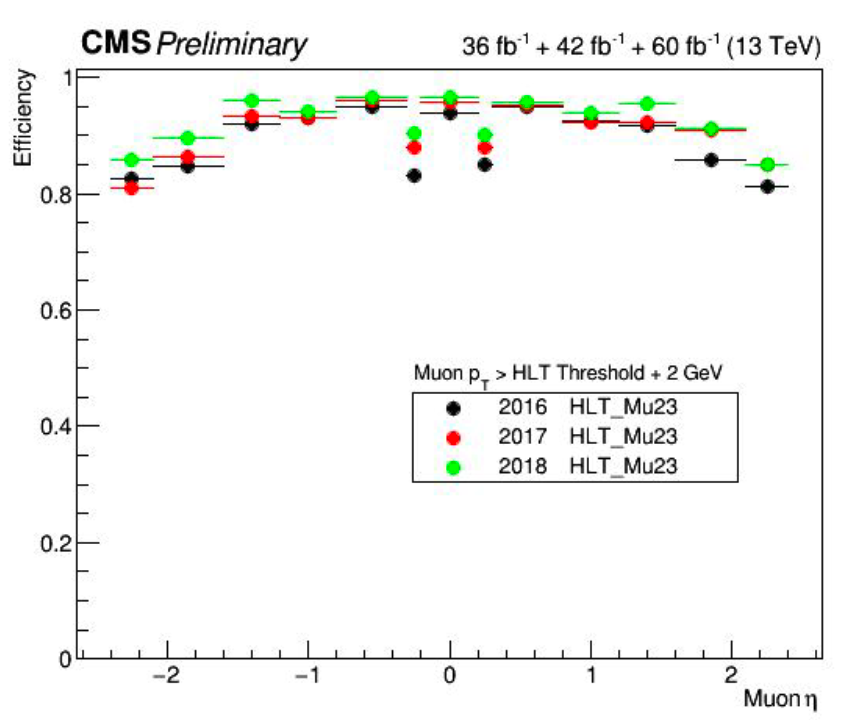
\includegraphics[width=1.0\textwidth]{figures/ch-5-object-reconstruction-and-corrections-applied/muon_efficiency_vs_eta_emu_HLT_Mu23_TrkIsoVVL_Ele12_CaloIdL_TrackIdL_IsoVL_DZ.png}
        \caption{Muon efficiency vs. $\eta$.}
        \label{fig:muon_efficiency_vs_eta_emu}
    \end{subfigure}
    \caption[Efficiencies of the electron leg vs. $p_{T}$ (\textit{left}) and the muon log vs. $\eta$ (\textit{right}), for the HLT path with online thresholds of 12 GeV for the electron and 23 GeV for the muon, with the data-taking years 2016 through 2018 overlaid.]{Efficiencies of the electron leg vs. $p_{T}$ (\textit{left}) and the muon log vs. $\eta$ (\textit{right}), for the HLT path with online thresholds of 12 GeV for the electron and 23 GeV for the muon, for the data-taking years 2016 (\textit{black}), 2017 (\textit{red}), and 2018 (\textit{green}) \cite{CMS-DP-2019-025}.} 
\end{figure}


\subsection{Electrons and muons faking $\tau_{h}$: energy scales}

Energy scales for electrons misidentified as hadronic tau decays ($e$ faking $\tau_{h}$) are provided by the Tau POG, and were measured in the $e\tau_{h}$ channel with the visible invariant mass of the electron and hadronic tau system \cite{twiki_HiggsToTauTauWorkingLegacyRun2}. This energy scale is applied for $\tau_{h}$ with $p_{T} > 20$ GeV regardless of which DeepTau vs. electron working point was used. Values for 2018 are shown in Table \ref{table:electron-faking-tauh-FES-2018}.

% root -l TauFES_eta-dm_DeepTau2017v2p1VSe_2018ReReco.root 
\begin{table}[h]
    \centering
    \begin{tabular}{|c|c|}
    \hline
    \multicolumn{2}{|c|}{Electrons faking $\tau_{h}$ energy scale factor in 2018}      \\ \hline
    \hline
    Reconstructed decay mode of the fake $\tau_{h}$  & Central value and (up, down) shifts \\ \hline
    0   & 1.01362 (+0.00474, -0.00904) \\
    1   & 1.01945 (+0.01598, -0.01226) \\
    10  & 0.96903 (+0.0125, -0.03404) \\
    11 & 0.985 (+0.04309, -0.05499) \\ \hline
    \end{tabular}
    \caption[Energy scales and up/down systematic uncertainties applied to electrons misidentified as hadronic taus.]{Energy scales and up/down systematic uncertainties applied to electrons misidentified as hadronic taus for 2018, binned in decay mode of the fake $\tau_{h}$ \cite{twiki_HiggsToTauTauWorkingLegacyRun2}.}
    \label{table:electron-faking-tauh-FES-2018}
\end{table}

No nominal energy scale is applied for muons mis-reconstructed as $\tau_{h}$, and the uncertainty is treated as $\pm$ 1\% and uncorrelated in the reconstructed decay mode \cite{twiki_HiggsToTauTauWorkingLegacyRun2}. 

\subsection{Electrons and muons faking $\tau_{h}$: misidentification efficiencies}
Corrections on identification efficiencies are applied to genuine electrons and muons misidentified as $\tau$ to account for differences in data and MC.

The specific values depend on the vs. electron and vs. muon discriminator working points used. 
For misidentified $\mu \rightarrow \tau_{h}$, the scale factors are split into different $|\eta|$ regions, determined by the CMS muon and tracker detector geometries, as shown in Table \ref{table:tauIDeff_deepTau_vs_muon} for 2018 \cite{twiki_TAU_POG_tauidrecommendationforrun2}.


\begin{table}[h]
    \centering
    \begin{tabular}{|c|c|c|}
    \hline
    \multicolumn{3}{|c|}{Tau ID efficiency for DeepTau vs. muon WPs in 2018} \\ \hline
    \hline
    $|\eta|$  & Tight working point & VLoose working point \\ \hline
    (0.0, 0.2)     & 0.767 $\pm$ 0.127  & 0.954 $\pm$ 0.069  \\ \hline 
    (0.2, 0.6)     & 1.255 $\pm$ 0.258  & 1.009 $\pm$ 0.098  \\ \hline 
    (0.6, 1.0)     & 0.902 $\pm$ 0.203  & 1.029 $\pm$ 0.075 \\ \hline 
    (1.0, 1.45)    & 0.833 $\pm$ 0.415  & 0.928 $\pm$ 0.145\\ \hline
    (1.45, 2.0)    & 4.436 $\pm$ 0.814   & 5.000 $\pm$ 0.377 \\ \hline
    (2.0, 2.53)    & 1.000 $\pm$ 0.000         & 1.000 $\pm$ 0.000\\ \hline
    \end{tabular}
    \caption[Tau mis-identification efficiency for the DeepTau Tight and Very Loose (VLoose) working points vs. muons in 2018.]{Tau mis-identification efficiency for the DeepTau Tight and Very Loose (VLoose) working points vs. muons in 2018, binned in the muon $|\eta|$ \cite{twiki_TAU_POG_tauidrecommendationforrun2}.}
    \label{table:tauIDeff_deepTau_vs_muon}
\end{table}

For misidentified $e \rightarrow \tau_{h}$, the scale factors are split into barrel and endcap regions, dictated by the ECAL detector geometry, as shown in Table \ref{table:tauIDeff_deepTau_vs_electron} for 2018.

% root -l /Users/stephaniekwan/Dropbox/Princeton_G6/TauIDSFs/data/TauID_SF_eta_DeepTau2017v2p1VSe_2018ReReco.root 
\begin{table}[h]
    \centering
    \begin{tabular}{|c|c|c|}
    \hline
    \multicolumn{3}{|c|}{Tau ID efficiency for DeepTau vs. electron WPs in 2018} \\ \hline
    \hline
    $|\eta|$  & Tight working point & VLoose working point \\ \hline
    (0.0, 0.73)     & 1.47 $\pm$ 0.27  & 0.95 $\pm$ 0.07  \\ \hline 
    (0.73, 1.509)   & 1.509 $\pm$ 0.0  & 1.00 $\pm$ 0.0  \\ \hline 
    (1.509, 1.929)  & 1.929 $\pm$ 0.2  & 0.86 $\pm$ 0.1 \\ \hline 
    (1.929, 2.683)  & 2.683 $\pm$ 0.9  & 2.68 $\pm$ 0.0 \\ \hline
    \end{tabular}
    \caption[Tau mis-identification efficiency for the DeepTau Tight and Very Loose (VLoose) working points vs. electrons in 2018.]{Tau mis-identification efficiency for the DeepTau Tight and Very Loose (VLoose) working points vs. electrons in 2018, binned in the electron $|\eta|$ \cite{twiki_TAU_POG_tauidrecommendationforrun2}.}
    \label{table:tauIDeff_deepTau_vs_electron}
\end{table}


\subsection{Electron ID and tracking efficiency}
Scale factors are applied to MC to correct for differences between MC and data in the performance of electron identification (ID) and tracking.

Electron and photon identification, as discussed earlier, use variables with good signal vs. background discrimination power such as lateral shower shape and ratio of energy deposited in the HCAL to energy deposited in the ECAL at the position of the electron. The cut-based electron identification efficiencies in data and ratio of efficiencies in data to MC are shown in Fig. \ref{fig:electron_MVA_ID_efficiency} for the multivariate analysis (MVA) identification working point. 

The tracking efficiencies in data and the data/MC ratio are shown in Fig. \ref{fig:electron_GSF_tracking_efficiency} for the Gaussian-sum filter (GSF) tracking \cite{CMS-DP-2020-037}. 

\begin{figure}[h]
    \centering
    \begin{subfigure}{0.45\textwidth}
        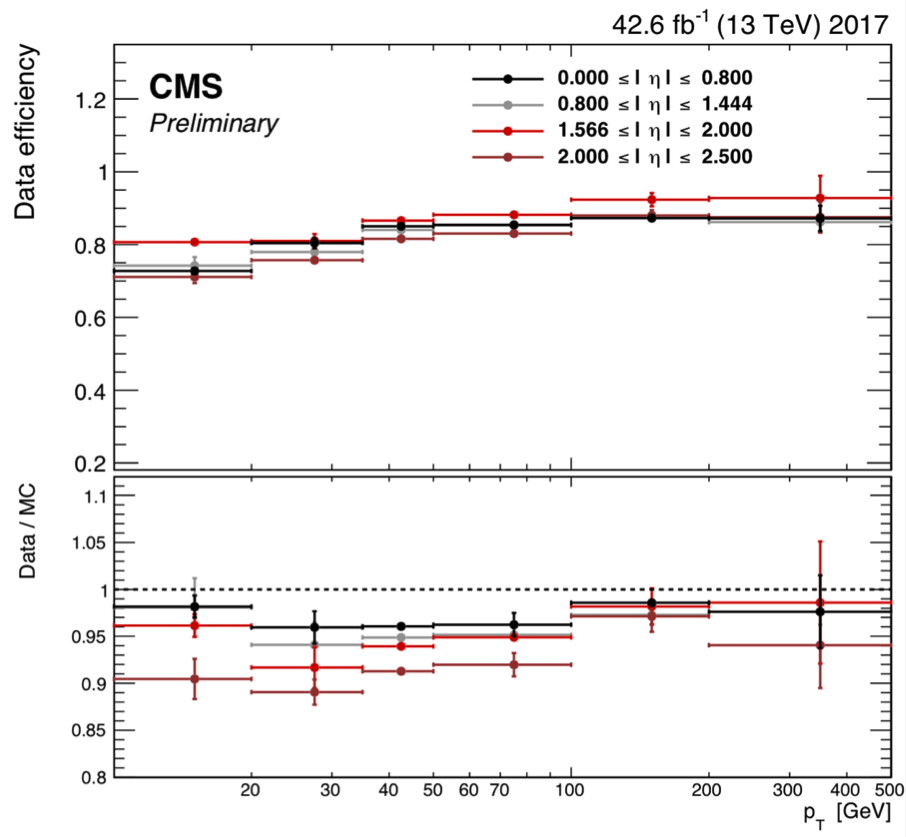
\includegraphics[width=1.0\textwidth]{figures/ch-5-object-reconstruction-and-corrections-applied/electron_MVA_90wp_identification_efficiency}
        \caption{Electron MVA ID.}
        \label{fig:electron_MVA_ID_efficiency}
    \end{subfigure}
    \hfill
    \begin{subfigure}{0.45\textwidth}
        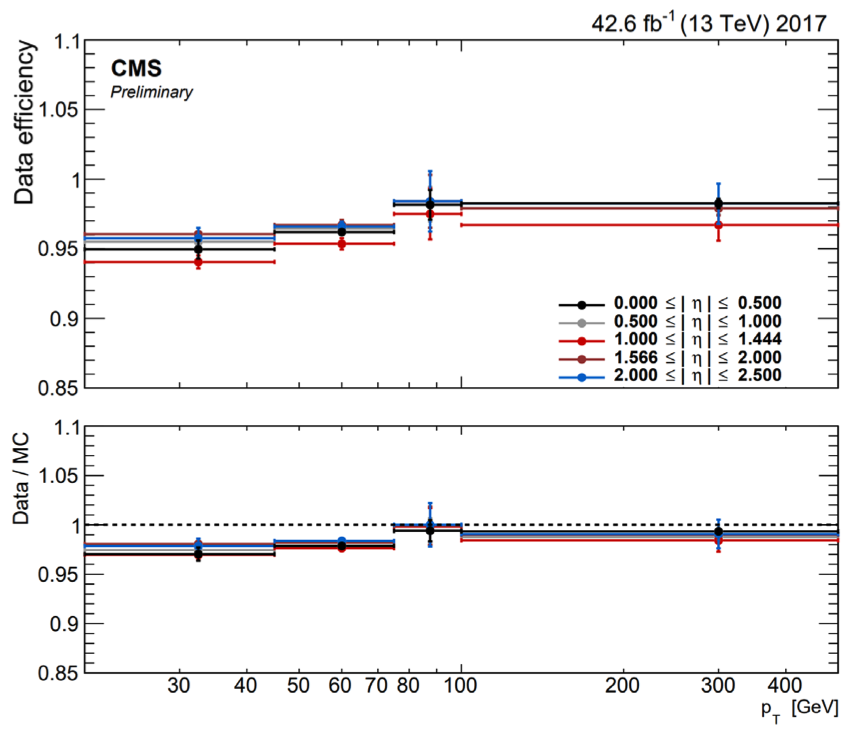
\includegraphics[width=1.0\textwidth]{figures/ch-5-object-reconstruction-and-corrections-applied/electron_gsf_tracking_efficiency}
        \caption{Electron GSF tracking.}
        \label{fig:electron_GSF_tracking_efficiency}
    \end{subfigure}
    \caption[Efficiencies in data (\textit{top panels}) and the ratio of efficiencies in data/MC (\textit{bottom panels}), for the electron multivariate analysis (MVA) identification (\textit{left}) and for the Gaussian-sum filter (GSF) tracking (\textit{right}).]{Efficiencies in data (\textit{top panels}) and the ratio of efficiencies in data/MC (\textit{bottom panels}), for the electron multivariate analysis (MVA) identification (\textit{left}) and for the Gaussian-sum filter (GSF) tracking (\textit{right}) \cite{CMS-DP-2020-037}. Error bars represent statistical and systematic uncertainties.} 
\end{figure}


\subsection{Muon ID, isolation, and tracking efficiencies}
Scale factors are applied to MC to correct for differences between MC and data in the performance of muon identification, isolation, and tracking, as detailed below.

The efficiencies for muon identification measured in 2015 data and MC simulation are shown in Figures \ref{fig:muon_looseID_efficiency} and \ref{fig:muon_tightID_efficiency} for the loose ID and tight ID respectively \cite{CMS-MUO-16-001}. The loose ID is chosen such that efficiency exceeds 99\% over the full $\eta$ range, and the data and simulation agree to within 1\%. The tight ID is chosen such that efficiency varies between 95\% and 99\% as a function of $\eta$, and the data and simulation agree to within 1-3\%. The muon identification working point used in this analysis is the medium ID, which has an efficiency of 98\% for all $\eta$ and an agreement within 1-2\% \cite{CMS-MUO-16-001}. 

\begin{figure}[h]
    \centering
    \begin{subfigure}{0.45\textwidth}
        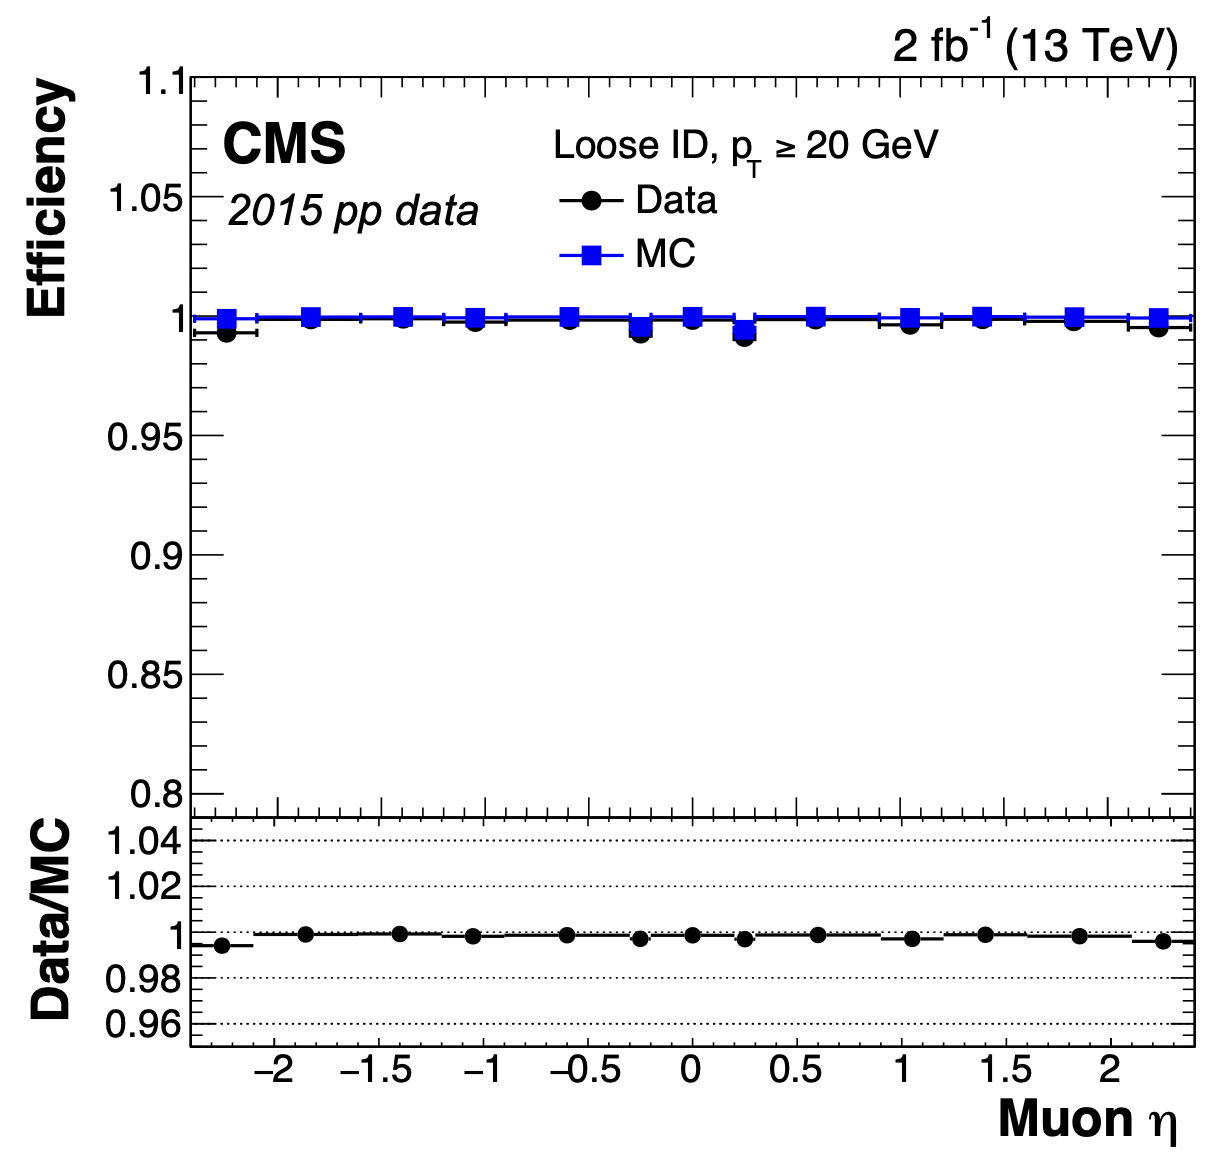
\includegraphics[width=1.0\textwidth]{figures/ch-5-object-reconstruction-and-corrections-applied/muon_efficiency_looseID}
        \caption{Muon efficiency isolation vs $p_{T}$.}
        \label{fig:muon_looseID_efficiency}
    \end{subfigure}
    \hfill
    \begin{subfigure}{0.45\textwidth}
        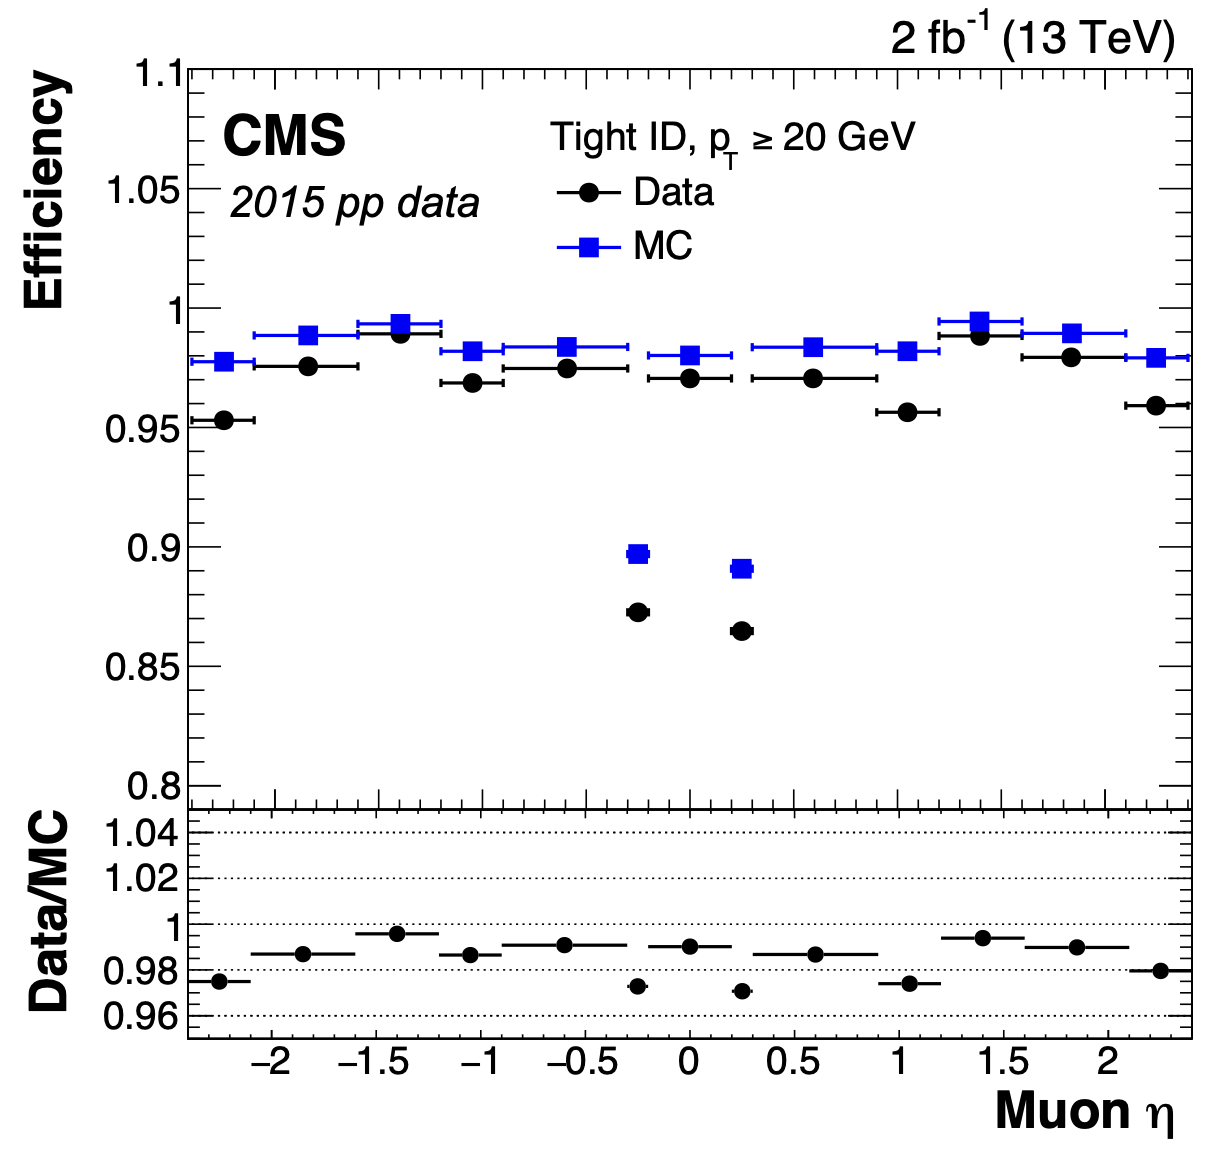
\includegraphics[width=1.0\textwidth]{figures/ch-5-object-reconstruction-and-corrections-applied/muon_efficiency_tightID}
        \caption{Muon isolation efficiency vs. $|\eta|$.}
        \label{fig:muon_tightID_efficiency}
    \end{subfigure}
    \caption[Muon identification efficiencies in 2015 data and MC as a function of the muon $p_{T}$ for the loose ID (\textit{left}) and tight ID (\textit{right}) working points.]{Muon identification efficiencies in 2015 data and MC as a function of the muon $p_{T}$ for the loose ID (\textit{left}) and tight ID (\textit{right}) working points \cite{CMS-MUO-16-001}.} 
\end{figure}

The efficiencies in data for the muon isolation, as measured in Level-3 muons (muons in one of the final stages of reconstruction in the HLT), as a function of the muon $p_{T}$ and $|\eta|$ are shown in Figures \ref{fig:muon_isolation_efficiency_vsPt} and \ref{fig:muon_isolation_efficiency_vsEta} \cite{CMS-MUO-16-001}. The HLT muon reconstruction consists of two steps: Level-2 (L2), where the muon is reconstructed in the muon subdetectors only, and Level-3 (L3) which is a global fit of tracker and muon hits (i.e. the global muon reconstruction as described in Section \ref{section:ch-5-muon-reconstruction}) \cite{Verwilligen-proceedings-2016}.

\begin{figure}[h]
    \centering
    \begin{subfigure}{0.45\textwidth}
        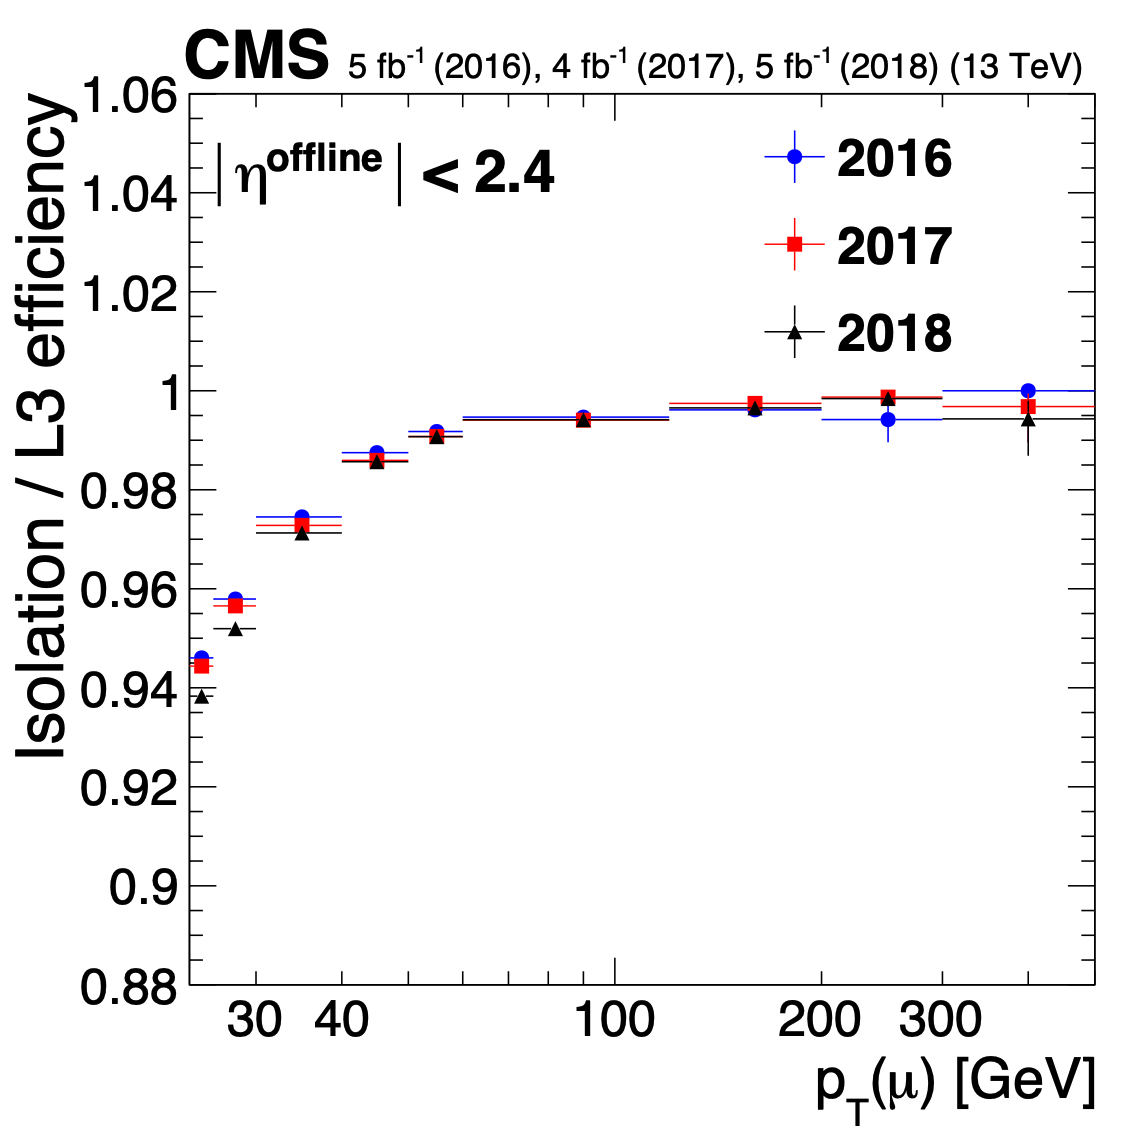
\includegraphics[width=1.0\textwidth]{figures/ch-5-object-reconstruction-and-corrections-applied/muon_efficiency_isolation_vsPt}
        \caption{Muon efficiency isolation vs $p_{T}$.}
        \label{fig:muon_isolation_efficiency_vsPt}
    \end{subfigure}
    \hfill
    \begin{subfigure}{0.45\textwidth}
        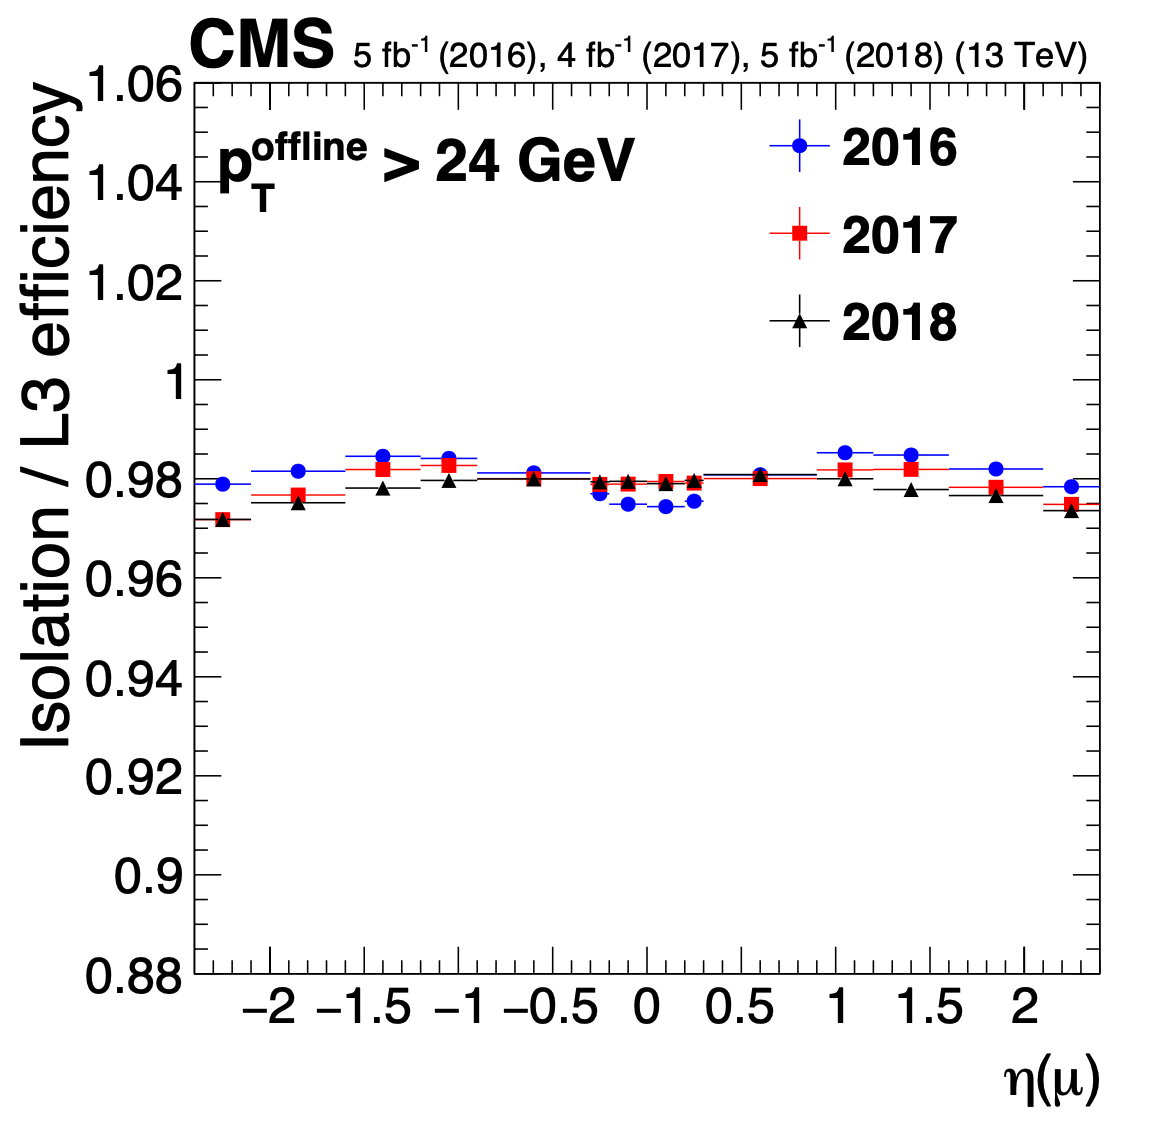
\includegraphics[width=1.0\textwidth]{figures/ch-5-object-reconstruction-and-corrections-applied/muon_efficiency_isolation_vsEta}
        \caption{Muon isolation efficiency vs. $|\eta|$.}
        \label{fig:muon_isolation_efficiency_vsEta}
    \end{subfigure}
    \caption[Muon isolation efficiencies in Run-2 data as a function of the muon $p_{T}$ (\textit{left}) and $|\eta|$ (\textit{right}).]{Muon isolation efficiencies in Run-2 data with respect to Level-3 muons (one of the final stages of HLT muon reconstruction) as a function of the muon $p_{T}$ (\textit{left}) and $|\eta|$ (\textit{right}) \cite{CMS-MUO-16-001}.} 
\end{figure}

The muon tracking efficiencies as a function of $|\eta|$ for standalone muons (i.e. tracks from only the muon system, i.e. DT, CSC, and RPC, as discussed in Section \ref{section:ch-5-muon-reconstruction}), is shown for data and simulated Drell-Yan samples in Fig. \ref{fig:muon_tracking_efficiency} \cite{CMS-DP-2020-035}. 

\begin{figure}[h]
    \centering
    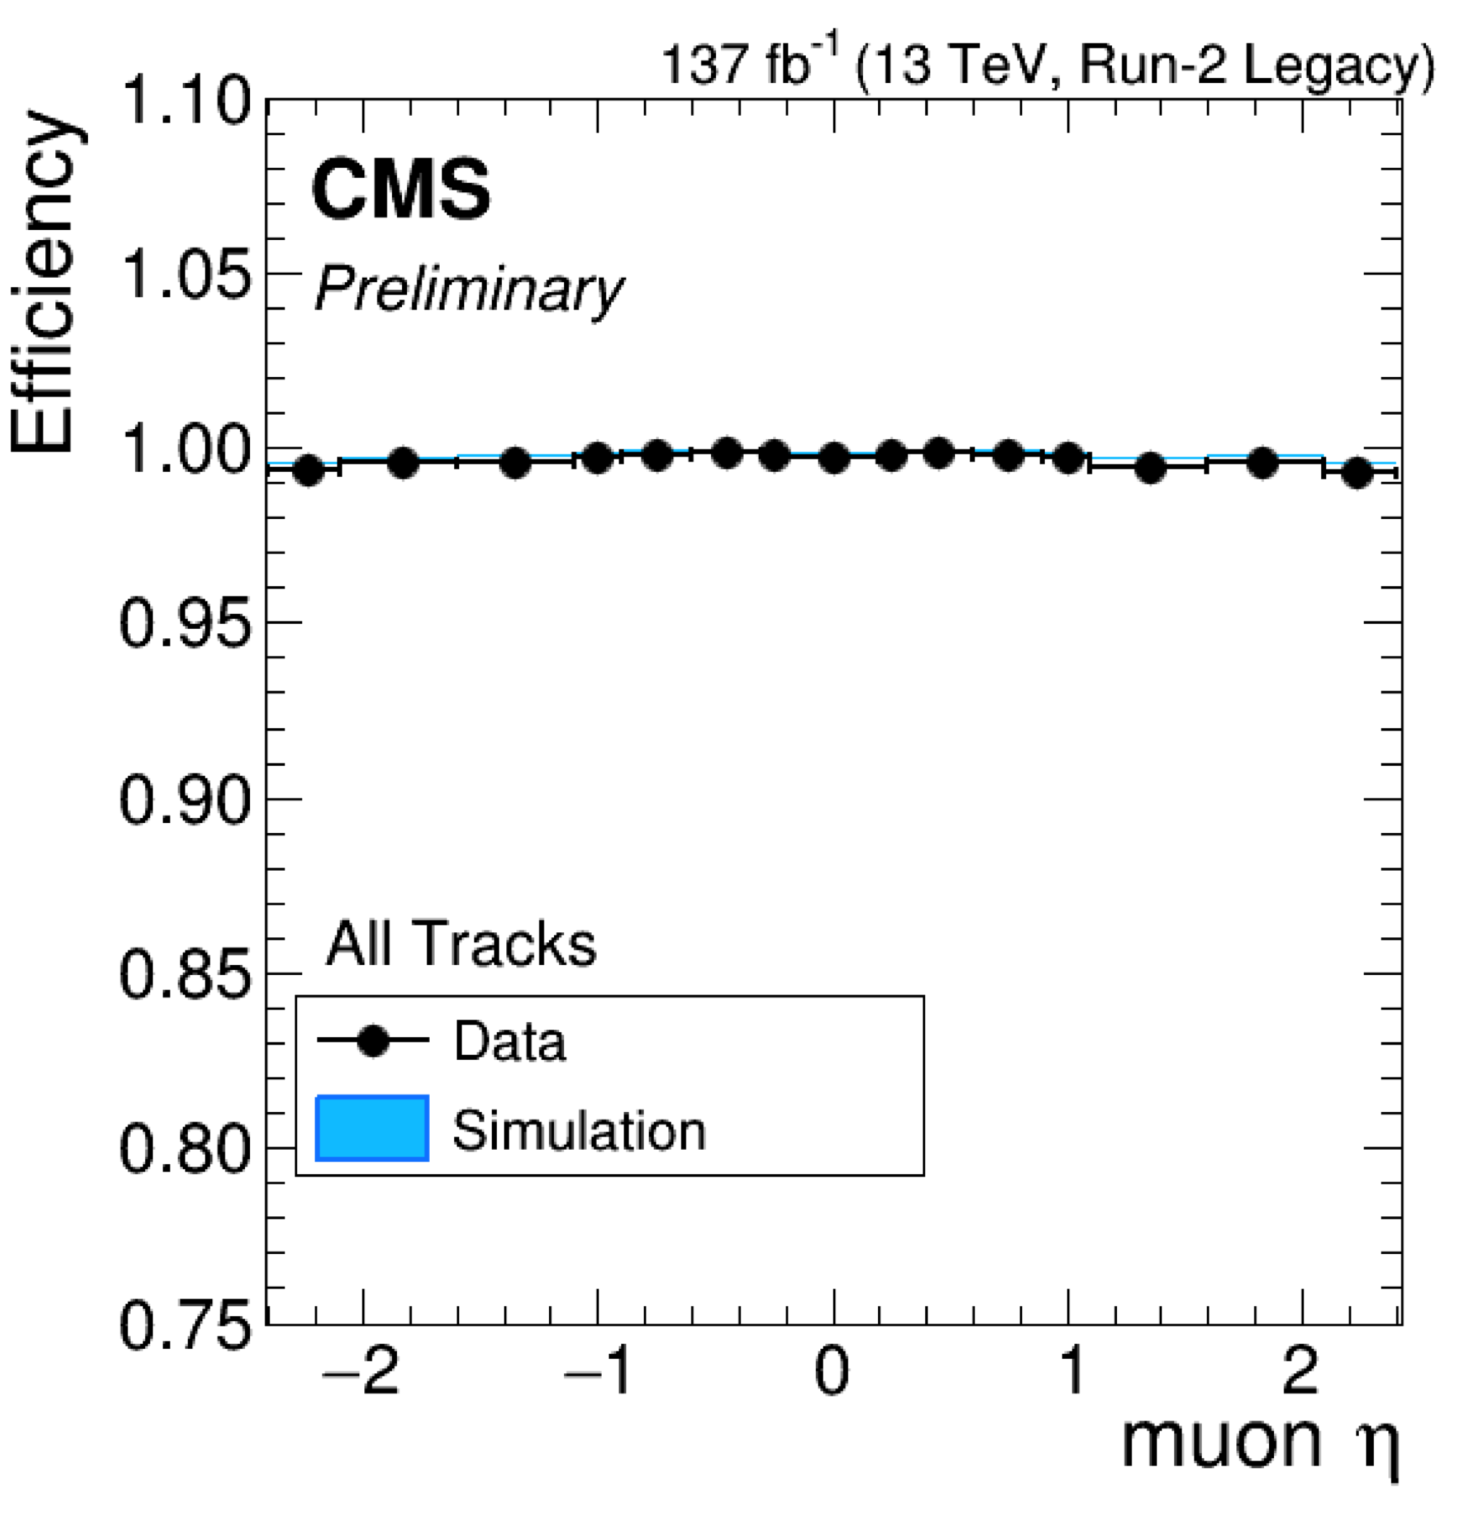
\includegraphics[width=8cm]{figures/ch-5-object-reconstruction-and-corrections-applied/muon_tracking_efficiency}
    \caption[Muon tracking efficiencies as a function of $|\eta|$ for standalone muons in Run-2 data (\textit{black}) and Drell-Yan (\textit{blue}) MC simulation.]{Muon tracking efficiencies as a function of $|\eta|$ for standalone muons in Run-2 data (\textit{black}) and Drell-Yan MC simulation (\textit{blue}) \cite{CMS-DP-2020-035}. All Tracks refers to tracks which exploit the presence of muon candidates in the muon system to seed the track reconstruction in the inner tracker, in contrast to tracks that use tracker-only hits for seeding. Uncertainties shown are statistical.}
    \label{fig:muon_tracking_efficiency}
\end{figure}

    

\subsection{Recoil corrections}
\label{sec:ch-8-recoil-corrections}
In proton-proton collisions, W and Z bosons are predominantly produced through quark-antiquark annihilation. Higher-order processes can induce radiated quarks or gluons that recoil against the boson, imparting a non-zero transverse momentum to the boson \cite{2009-Tevatron-recoil-correction}. Recoil corrections accounting for this effect are applied to samples with W+jets, Z+jets, and Higgs bosons \cite{twiki_HiggsToTauTauWorkingLegacyRun2}. The corrections are performed on the vectorial difference between the measured missing transverse momentum and the total transverse momentum of neutrinos originating from the decay of the W, Z, or Higgs boson. This vector is projected onto the axes parallel and orthogonal to the boson $p_{T}$. This vector, and the resulting correction to use, is measured in $Z \rightarrow \mu\mu$ events, since these events have leptonic recoil that do not contain neutrinos, allowing the 4-vector of the Z boson to be be measured precisely. The corrections are binned in generator-level $p_{T}$ of the parent boson and also the number of jets in the event.

\subsection{Drell-Yan corrections}
The Z boson transverse momentum distribution disagrees between leading-order (LO) simulations and data in a $Z \rightarrow \mu\mu$ control region with at least one b-tag jet \cite{CMS-HIG-17-024}. Per-event weights derived by the 2016 data-only version of this analysis \cite{CMS-HIG-17-024} are applied to $Z \rightarrow \tau\tau / \ell \ell$ events, as a function of the generator-level Z boson $p_{T}$ to provide better matching of MC to data.

\subsection{Pileup reweighing}
Reweighing is performed to rescale MC events to account for differences between MC and data, in the distribution of the pileup (number of additional proton-proton interactions per bunch crossing). A tool for calculating the pileup reweighing for the MC samples used is provided centrally by the Luminosity POG \cite{twiki_LUMI_POG_recommendation}.

\subsection{Pre-firing corrections}
In 2016 and 2017 data-taking, a gradual timing shift of ECAL was not properly propagated to L1 trigger primitives (TPs), resulting in a large fraction of high $\eta$ TPs being incorrectly associated with the previous bunch crossing. L1 trigger rules prevent two consecutive bunch crossings from firing, causing events to be rejected if significant ECAL energy was deposited in $2.0 < |\eta| 3.0$. To account for this issue, MC simulations for 2016 and 2017 are corrected using an event-dependent weight. Embedded samples are not corrected \cite{CMS-HIG-19-010}.

\subsection{Top $p_{T}$ spectrum reweighing}
In Run-1 and Run-2 it was observed that the $p_{T}$ spectra of top quarks in $t\bar{t}$ data was significantly softer than those predicted by MC simulations \cite{twiki_Top_pt_reweighing}. Possible sources of this discrepancy are higher order QCD and/or electroweak corrections, and non-resonant production of $t\bar{t}$-like final states. To account for this, corrections derived from Run-2 data by the Top Physics Analysis Group (PAG) are applied to the $p_{T}$ of the top and anti-top quarks in MC simulations, computed as a function of their generator-level $p_{T}$ \cite{twiki_Top_pt_reweighing}.

\subsection{B-tagging efficiency}
In order to predict correct b-tagging discriminant distributions and event yields in data, the weight of selected MC events is reweighed according to recommendations by the BTV POG \cite{twiki_btag_SF_methods}. The reweighing depends on the jet $p_{T}$, $\eta$, and the b-tagging discriminant. In this method, there is no migration of events from one b-tag multiplicity bin to another.

\subsection{Jet energy resolution and jet energy smearing}
Calibration of jet energies, i.e. ensuring that the energy and momentum of the reconstructed jet matches that of the quark/gluon-initiated jet, is a challenging task due to time-dependent changes in the detector response and calibration and high pileup \cite{CMS-JME-13-004} \cite{proceedings-Agarwal:2022txa}. Jet calibration is done via jet energy corrections (JECs) applied to the $p_{T}$ of jets in MC samples, accounting successively for the effects of pileup, uniformity of the detector response, and residual data-simulation jet energy scale differences \cite{twiki_JetResolution_JEC}. Typical jet energy resolutions reported at $\sqrt{s} = 8$ TeV in the central rapidities are 15-20\% at 30 GeV and about 10\% at 100 GeV \cite{CMS-JME-13-004}. Jet energy corrections are also propagated to the missing transverse energy.

Measurements show that the jet energy resolution (JER) in data is worse than in simulation, and so the jets in MC need to be smeared to describe the data. JER corrections are applied after JEC on MC simulations, and adjust the width of the $p_{T}$ distribution based on pileup, jet size, and jet flavour \cite{twiki_JetResolution_JER}. Tools for applying JEC and JER are provided centrally by the JER Corrections group. 